\documentclass[pdftex,12pt,a4paper]{article}
\usepackage[pdftex]{graphicx}
\newcommand{\HRule}{\rule{\linewidth}{0.5mm}}
\usepackage{lipsum}
%\usepackage[utf8]{inputenc}
\usepackage[a4paper,margin=2.5cm]{geometry}  
\usepackage{graphicx}% allows you to import images
\usepackage{caption}
\usepackage{subcaption}
\usepackage{float}
\usepackage{wallpaper}

\usepackage[hidelinks]{hyperref}  
%\usepackage{enumitem}
\usepackage{enumerate}
\usepackage{listings}
\usepackage{xcolor}
\usepackage{lipsum}
\usepackage{lmodern}
\usepackage{tcolorbox}
\usepackage{setspace}
\renewcommand{\baselinestretch}{1.1}
%bullet preamlbe
\renewcommand{\labelitemi}{$\bullet$}
\renewcommand{\labelitemii}{$\diamond$}
\renewcommand{\labelitemiii}{$\circle$}
\renewcommand\thesection{\Roman{section}} 
\usepackage{mhchem} % allow us to write chemistry equation
%\usepackage{xfrac}  % allow for slanted fractions
%\usepackage{amsmath}
\usepackage{amssymb}
\usepackage{wasysym}
\usepackage{pifont}
\usepackage{multirow}
\usepackage[makeroom]{cancel}
\usepackage[numbers]{natbib}
\bibliographystyle{unsrt}
\citestyle{IEEEtran}

% shortcut
\def\be{\begin{equation}}
\def\ee{\end{equation}}
\def\bd{\begin{displaymath}}
\def\ed{\end{displaymath}}
\def\bi{\begin{itemize}}
\def\ei{\end{itemize}}
\def\bn{\begin{enumerate}}
\def\en{\end{enumerate}}
\def\ba{\begin{eqnarray*}}
\def\ea{\end{eqnarray*}}
\def\u{\text}  
\def\v{\mathbf}   
\def\^{\textsuperscript}
\def\_{\textsubscript}
\def\inf{\infty}
\def\bf{\textbf}
\lstset{language=Matlab}
\lstset{breaklines}
\lstset{extendedchars=false}
\usepackage{romannum}
% Romannum page number
\usepackage{fancyhdr}
\pagestyle{fancy}
\rhead{ELEN90053}
\lhead{\scriptsize  \textcopyright \quad Rui YUAN}

\begin{document}
\graphicspath{{./figs/}}
\begin{titlepage}
\begin{center}
% Upper part of the page
\begin{figure}[H]
      
\includegraphics[width=6cm]{logo.png}
    \end{figure}
	
	
	%------------------------------------------------
	%	Title
	%------------------------------------------------
	{\color[RGB]{0,0,128} {\huge University of Melbourne}\\[0.5\baselineskip] % Title line 1
		{\Huge ELEN90053 Electronic System Design  }\\[0.5\baselineskip] % Title line 2
		{\Huge WORKSHOP}}\\ % Title line 3}}
% Title
\vspace{0.05\textheight} % Whitespace between the rule and authors
\huge \bfseries SIMULATION REPORT
\rule{\textwidth}{1pt} % Thick horizontal rule
\vspace{0.02\textheight} % Whitespace between the rule and authors
% Author and supervisor
\begin{flushright} \large
Rui \textsc{YUAN}\\
813927 \\
\end{flushright}
\vfill
% Bottom of the page
\begin{flushright} \large
{\large \today}
\end{flushright}
\rule{\textwidth}{0.4pt} % Thin horizontal rule
	
	\vspace{2pt}\vspace{-\baselineskip} % Whitespace between rules
	
	\rule{\textwidth}{1pt} % Thick horizontal rule
\begin{flushright} \tiny
{\scriptsize  \textcopyright \quad Rui YUAN 2017-2019}
\end{flushright}
\end{center}
\end{titlepage}
\tableofcontents
%menu or not   
\newpage
\section{Over whole Front-End Schematics}
The whole circuit built as figure 1. 
\begin{figure}[H]
\centering
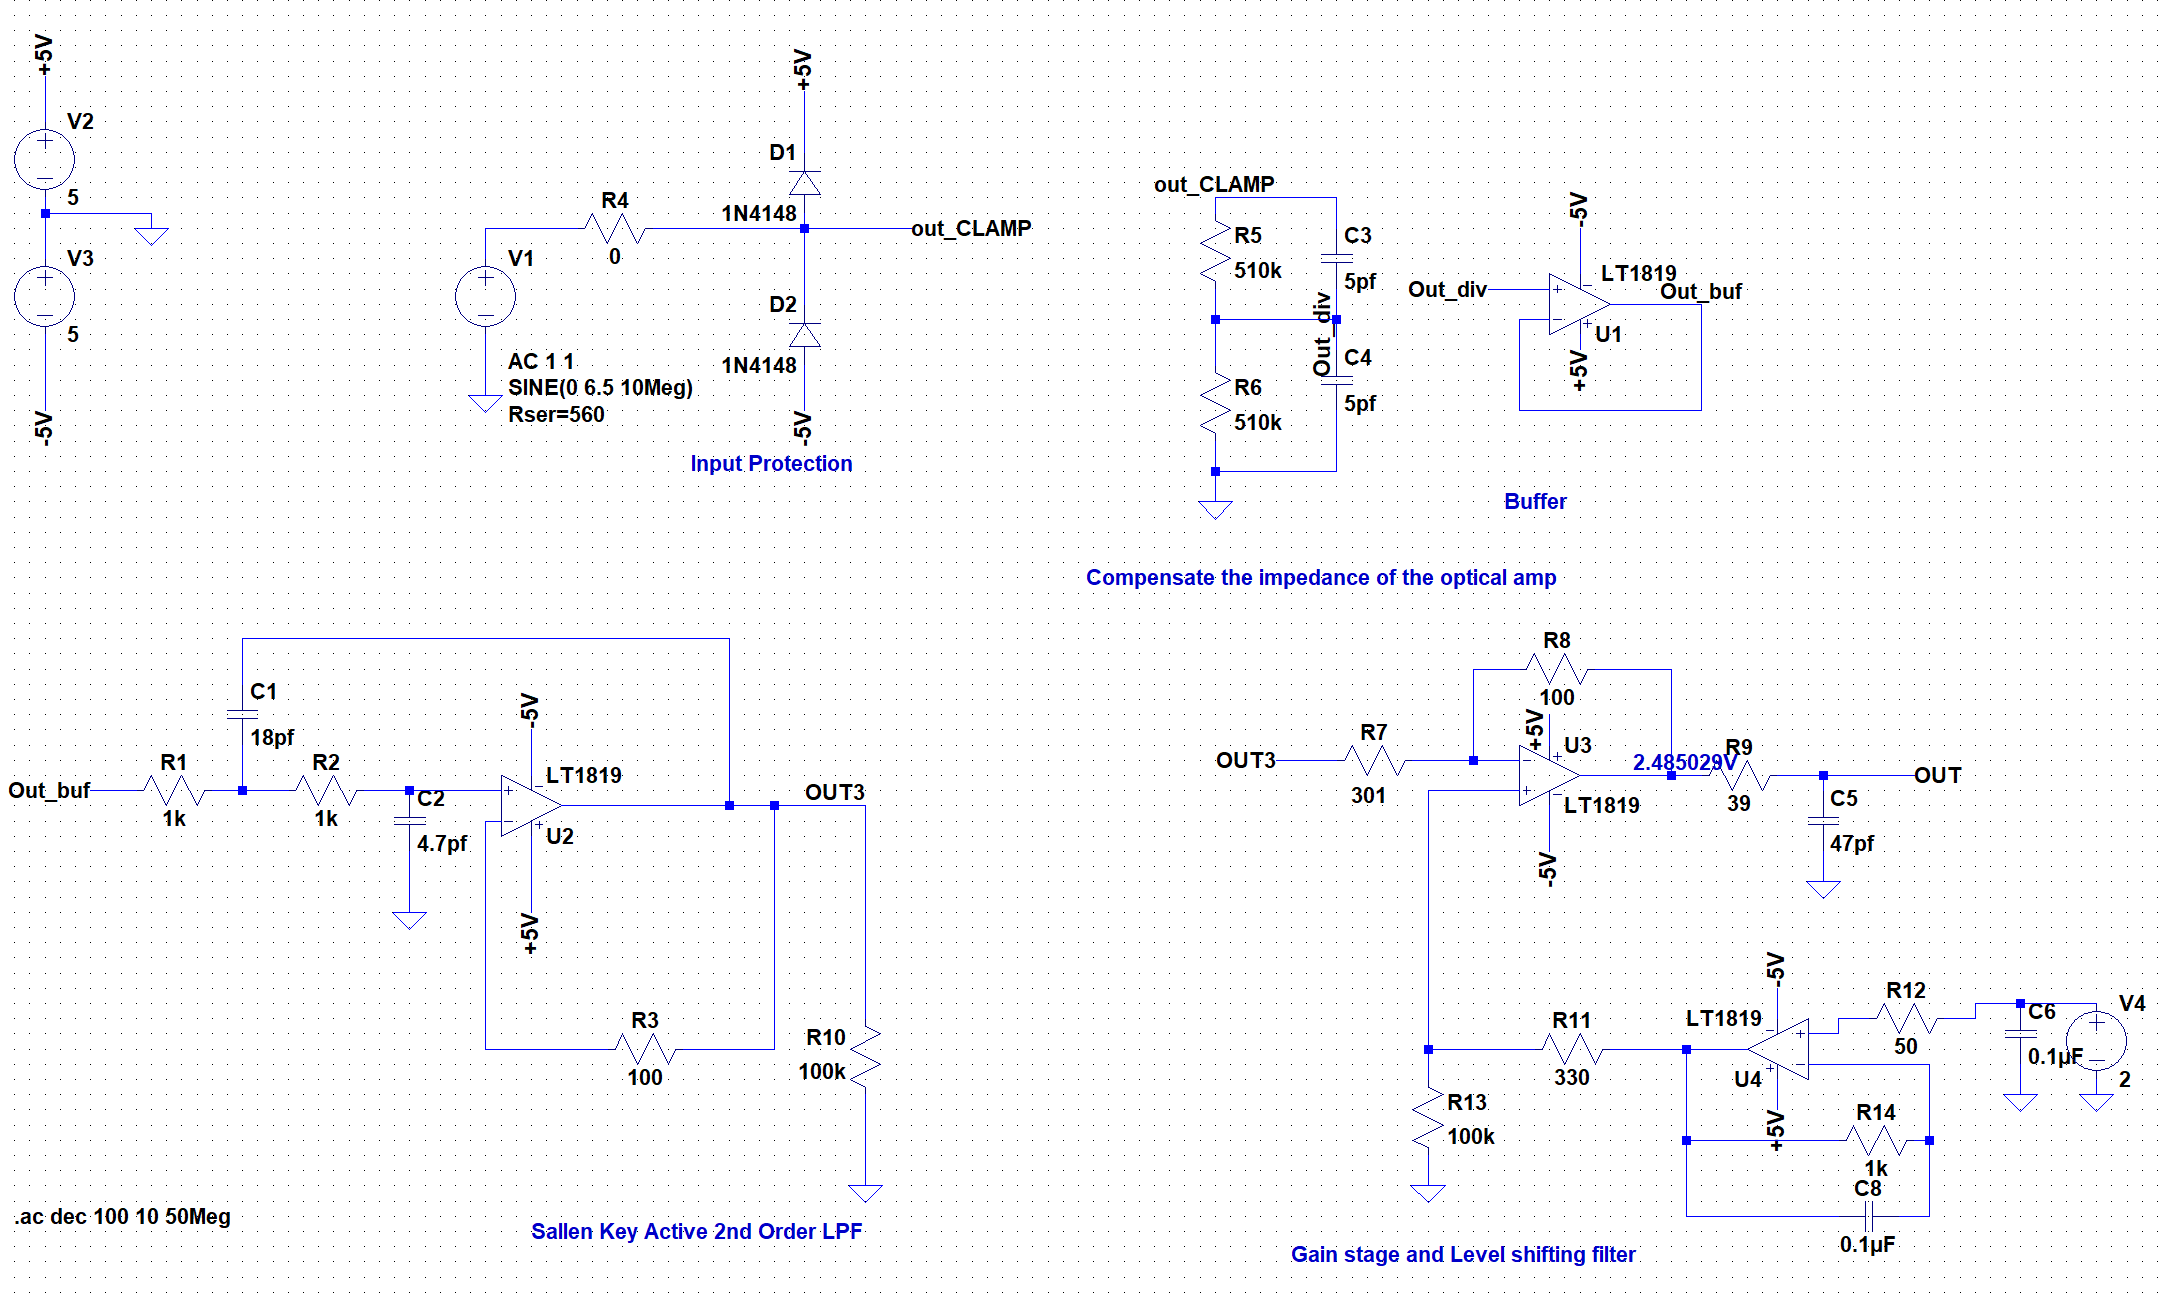
\includegraphics[width=16cm]{Sch.png}
\caption{The front end circuit designed}
\end{figure}
Each part will be discussed respectively at the sections
\section{Frequency and phase response graphs}
\begin{figure}[H]
\centering
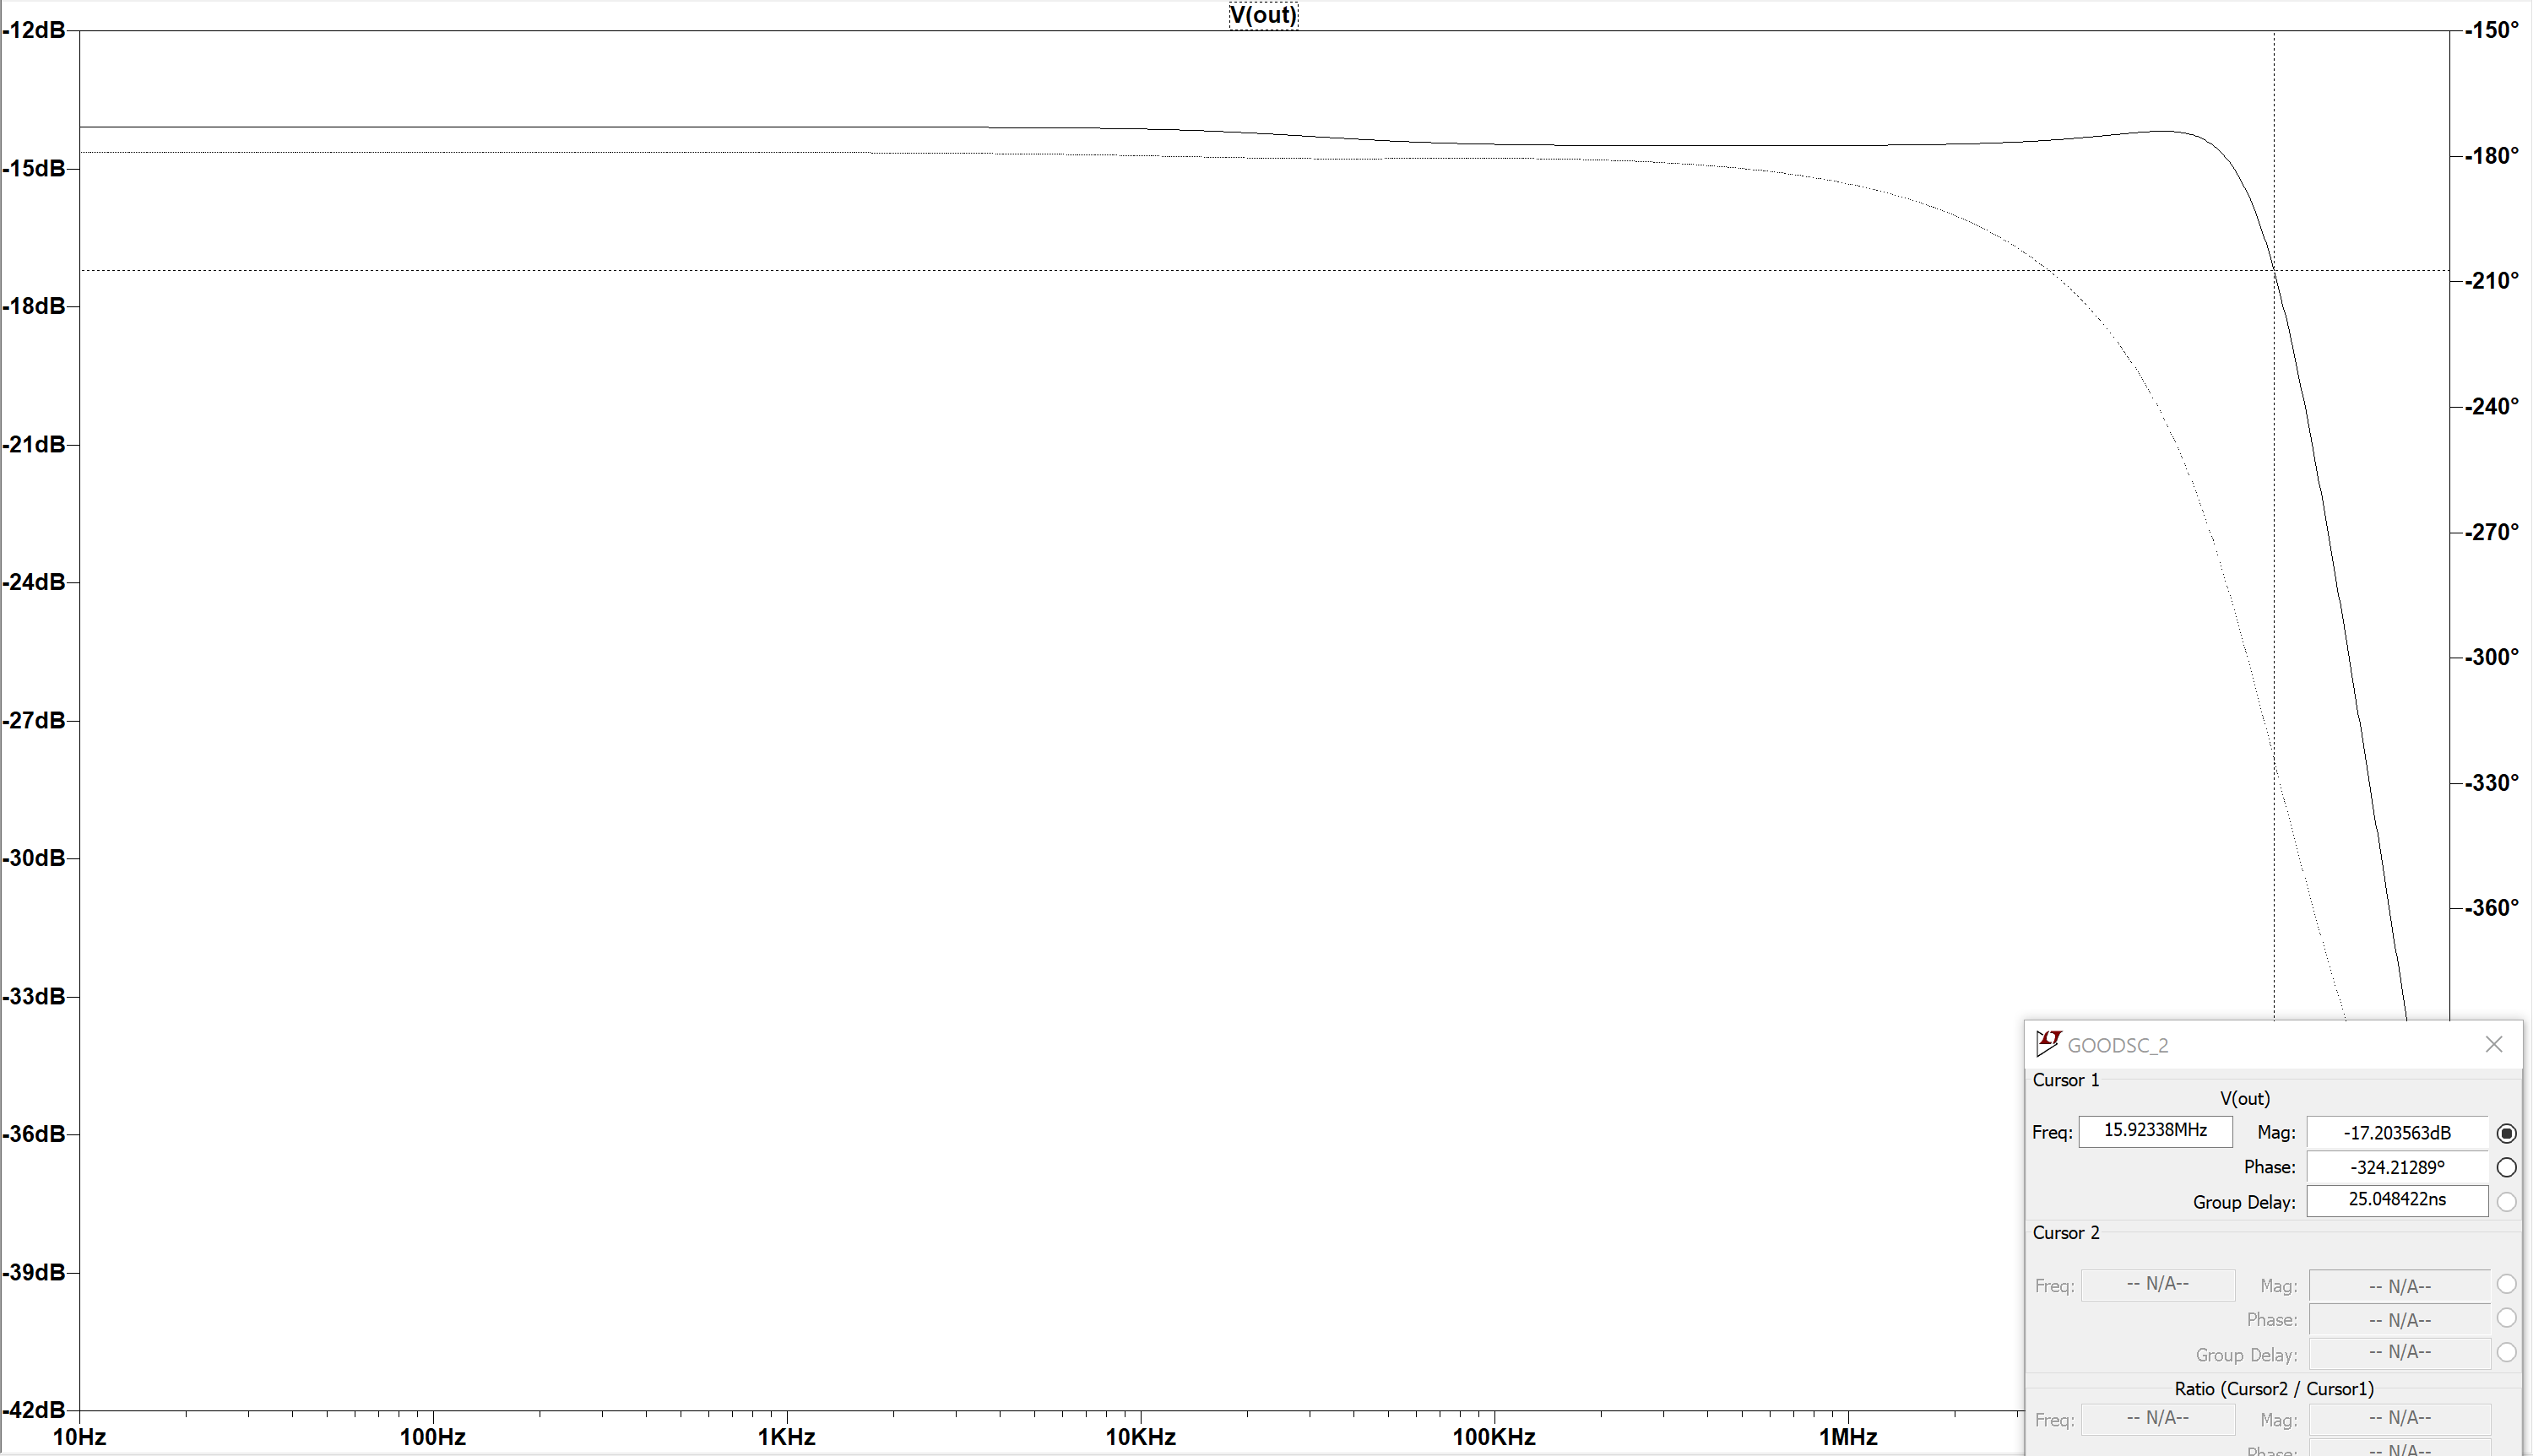
\includegraphics[width=14cm]{F-P-r.png}
\caption{Frequency and phase response at the ADC input}
\end{figure}
\begin{figure}[H]
\centering
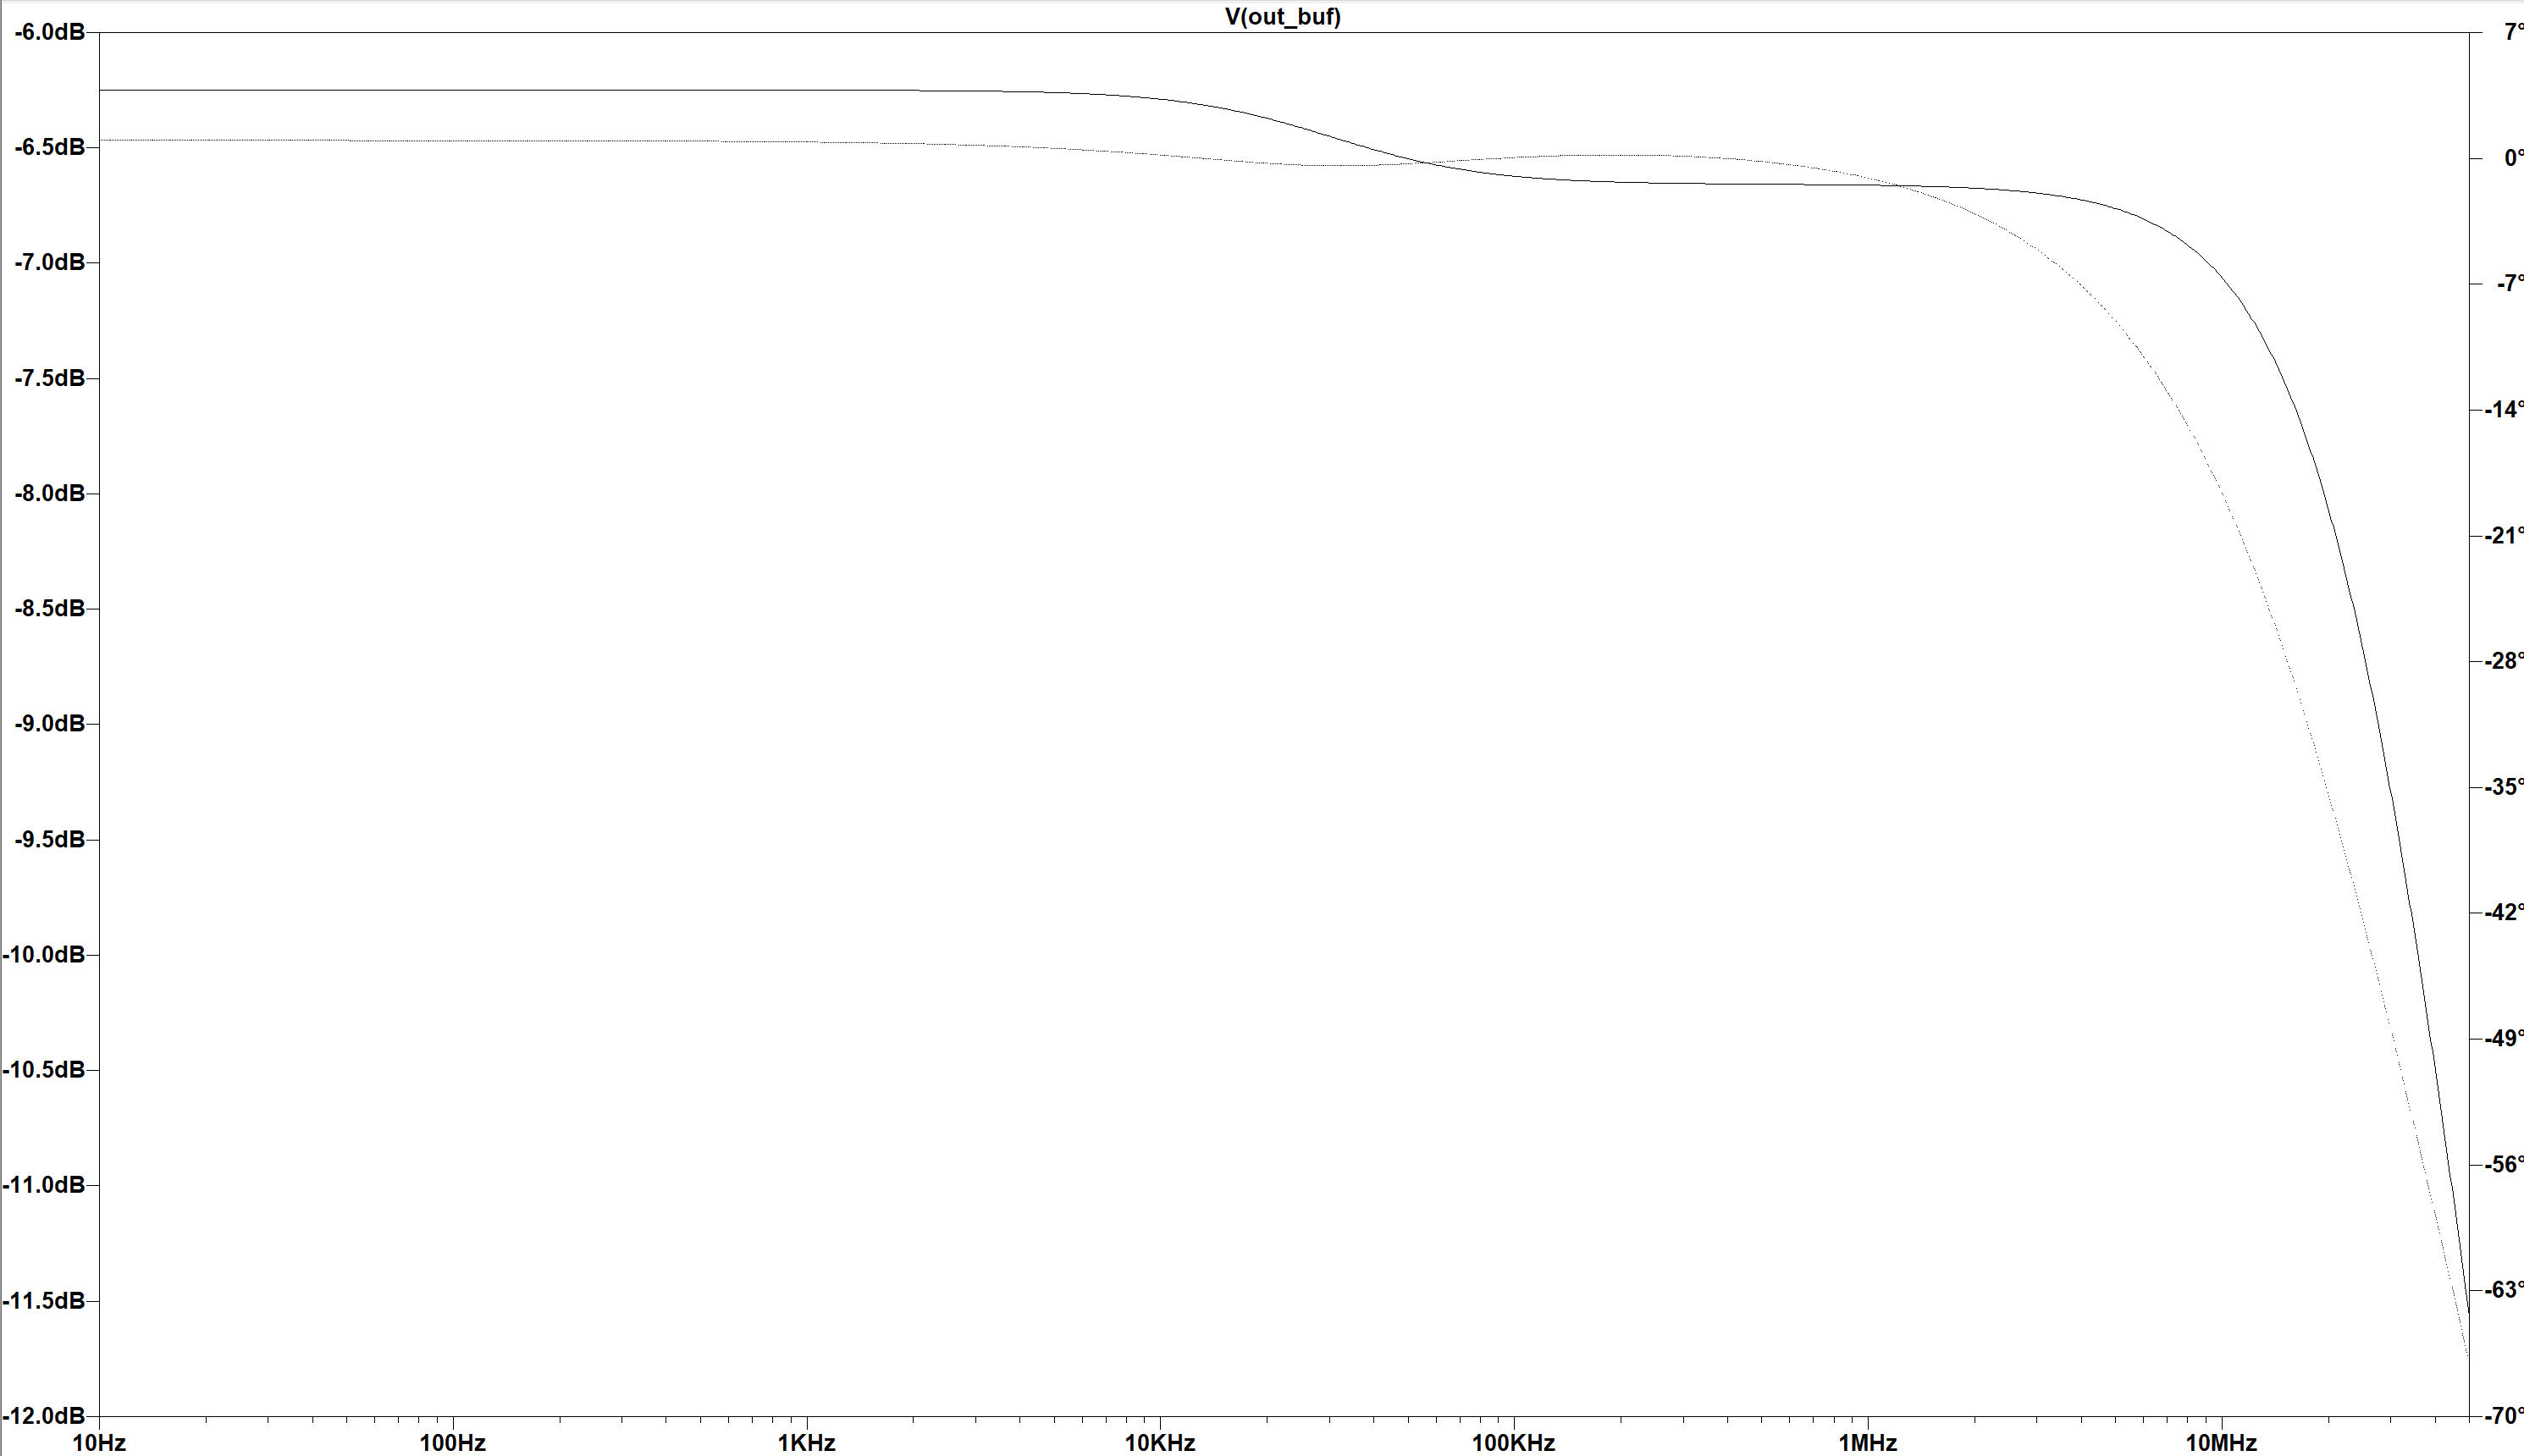
\includegraphics[width=14cm]{F-P-f.png}
\caption{Frequency and phase prior to the filter stage}
\end{figure}
From the figures above, the amplitude sent to adc has been decreased by $-14dB$, which is 0.199. This is designed intentionally as we want to shrink our amplitude from 10 V peak-to-peak to 2 V peak-to-peak. \textbf{While the phase has a 180 degree shift due to the feedback loop of the low pass filter, this can also be verified in figure 3}. The $-6dB$ amplitude decrease in figure 3 is discussed in section \Romannum{6}.
\section{Input impedance graph}
\begin{figure}[H]
\centering
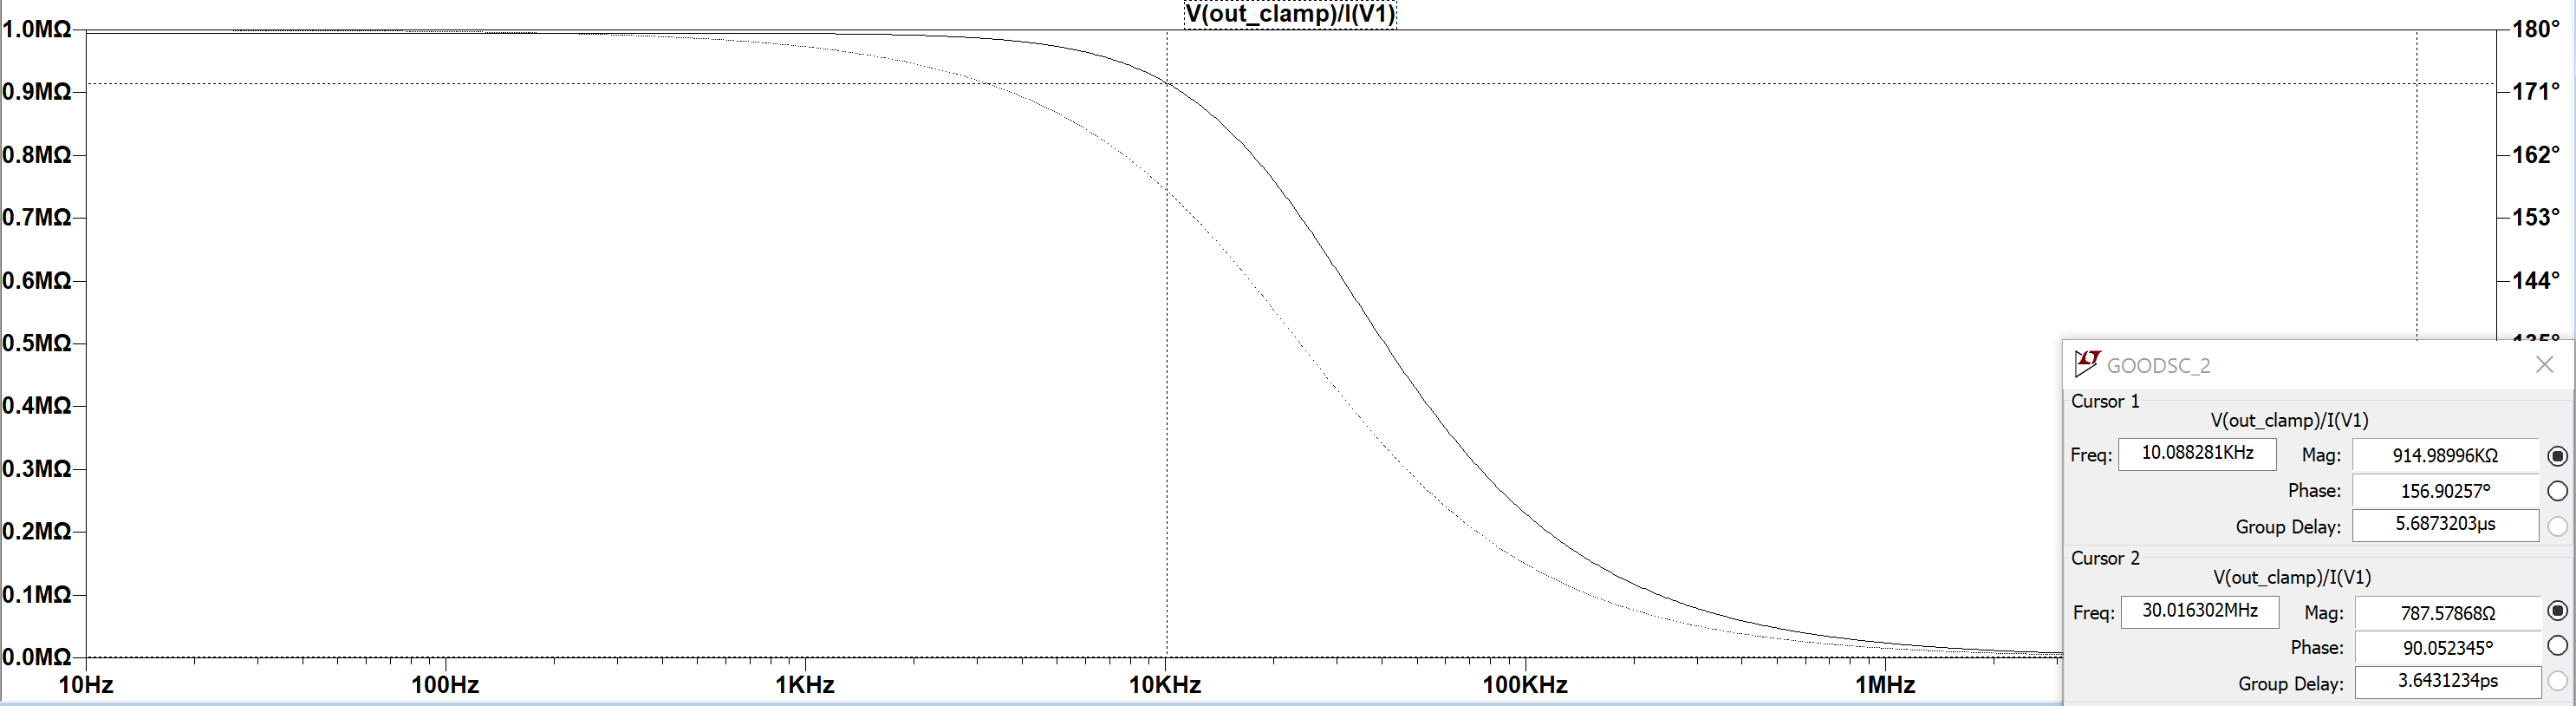
\includegraphics[width=14cm]{imp.png}
\caption{Input impedance measured at the BNC}
\end{figure}
~\\ From two cursors, the input impedance requirement is satisfied by the design. 
\section{Power dissipation table and DC bias}
The power consumption at each point collected as below:
\begin{table}[H]
\centering
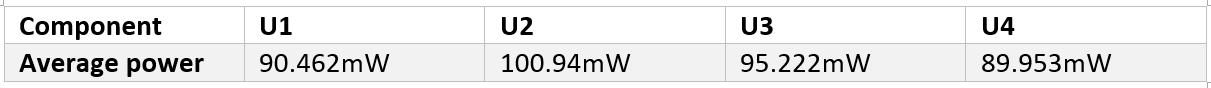
\includegraphics[width=12cm]{tab.png}
\caption{power consumption table}
\end{table} 
~\\Although all components' power seems in a reasonable range from the data sheet, to ensure all operational amplifiers running  well in the real circuit, currents of those amplifiers are measured as below: 
\begin{figure}[H]
\centering
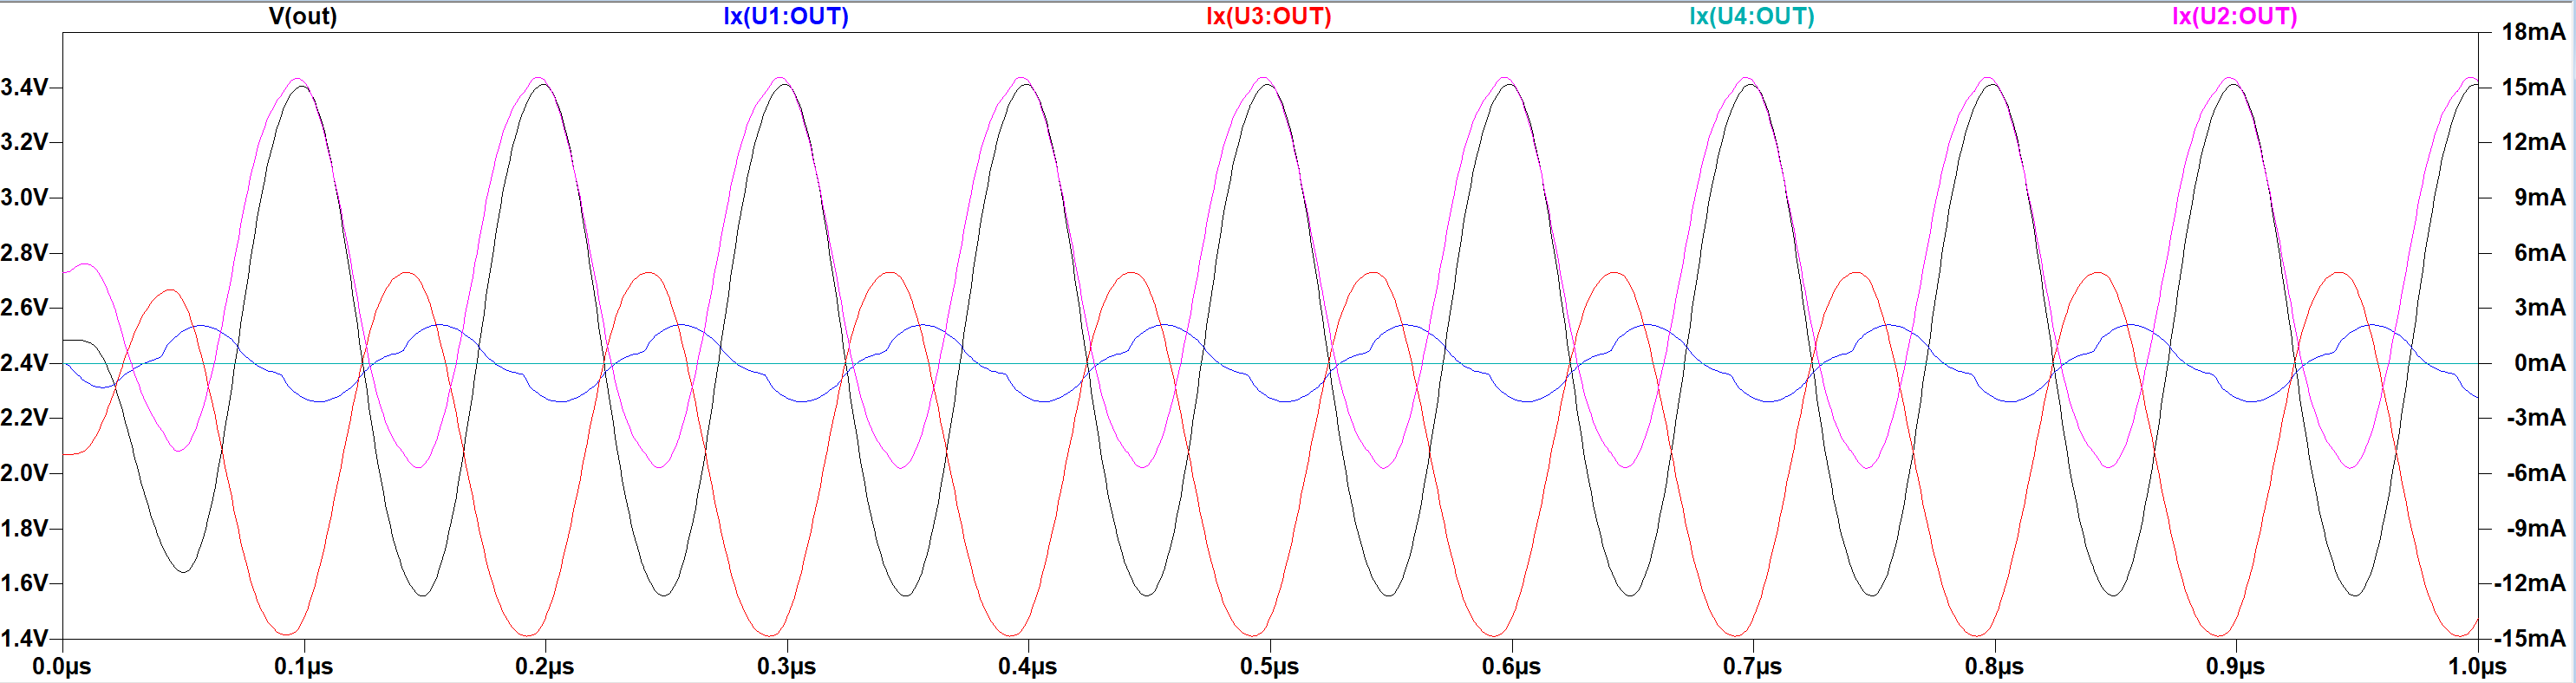
\includegraphics[width=16cm]{oplim.png}
\caption{Output current of each amplifier}
\end{figure}
~\\From data sheet, the maximum output current is $\pm 50mA$, from this circumstance, our design is safe as all the currents are within this range. \\
\textbf{The measured DC bias table is as below:} 
\begin{figure}[H]
\centering
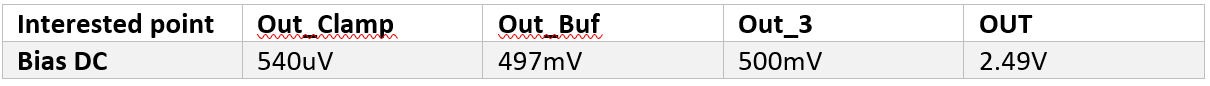
\includegraphics[width=16cm]{biasDC.png}
\caption{DC bias point of each stage.}
\end{figure}  
\section{Time domain plot for a 10Mhz input}
When a 10Mhz input signal with 5V amplitude is implemented, the output signal is as below:
\begin{figure}[H]
\centering
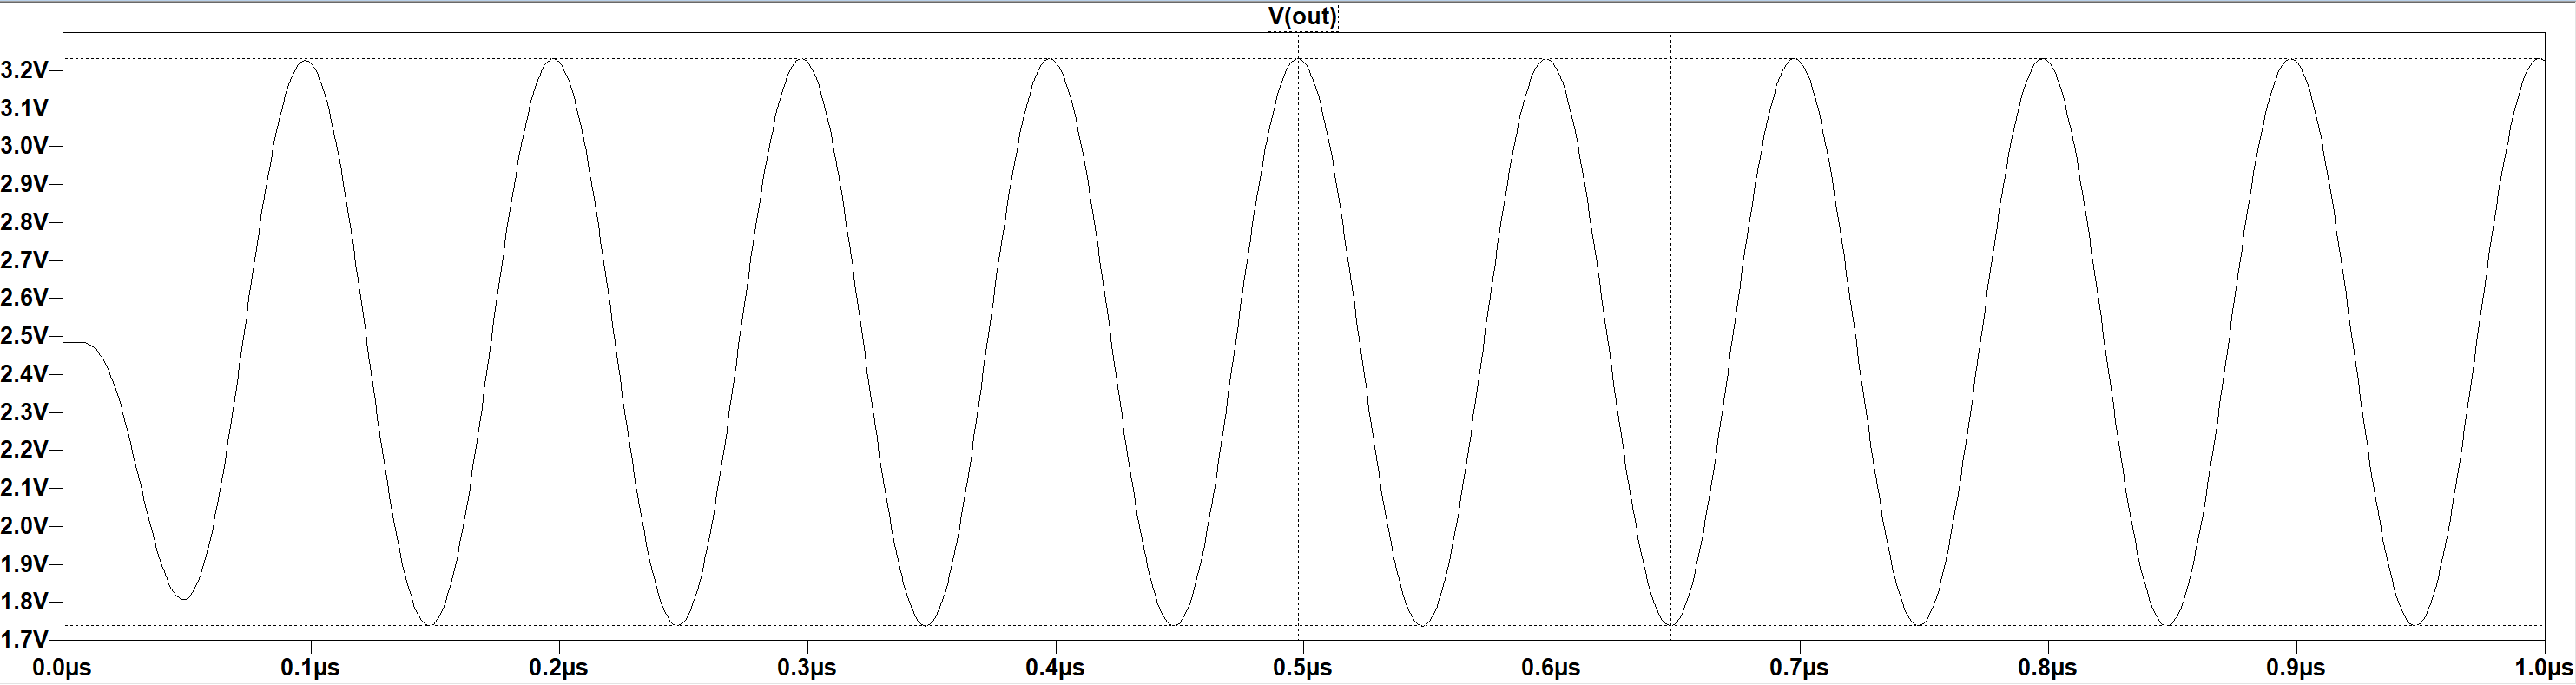
\includegraphics[width=16cm]{10M.png}
\caption{Input to the ADC when apply a 10Mhz input with 5V amplitude.}
\end{figure}
From the figure below, we can state the peak voltage of the output signal is from 1.7 to 3.3 centring around 2.5V. The amplitude is intentionally scale more than needed for the scenario when a large signal is clamped. This scenario is simulated as below:
\begin{figure}[H]
\centering
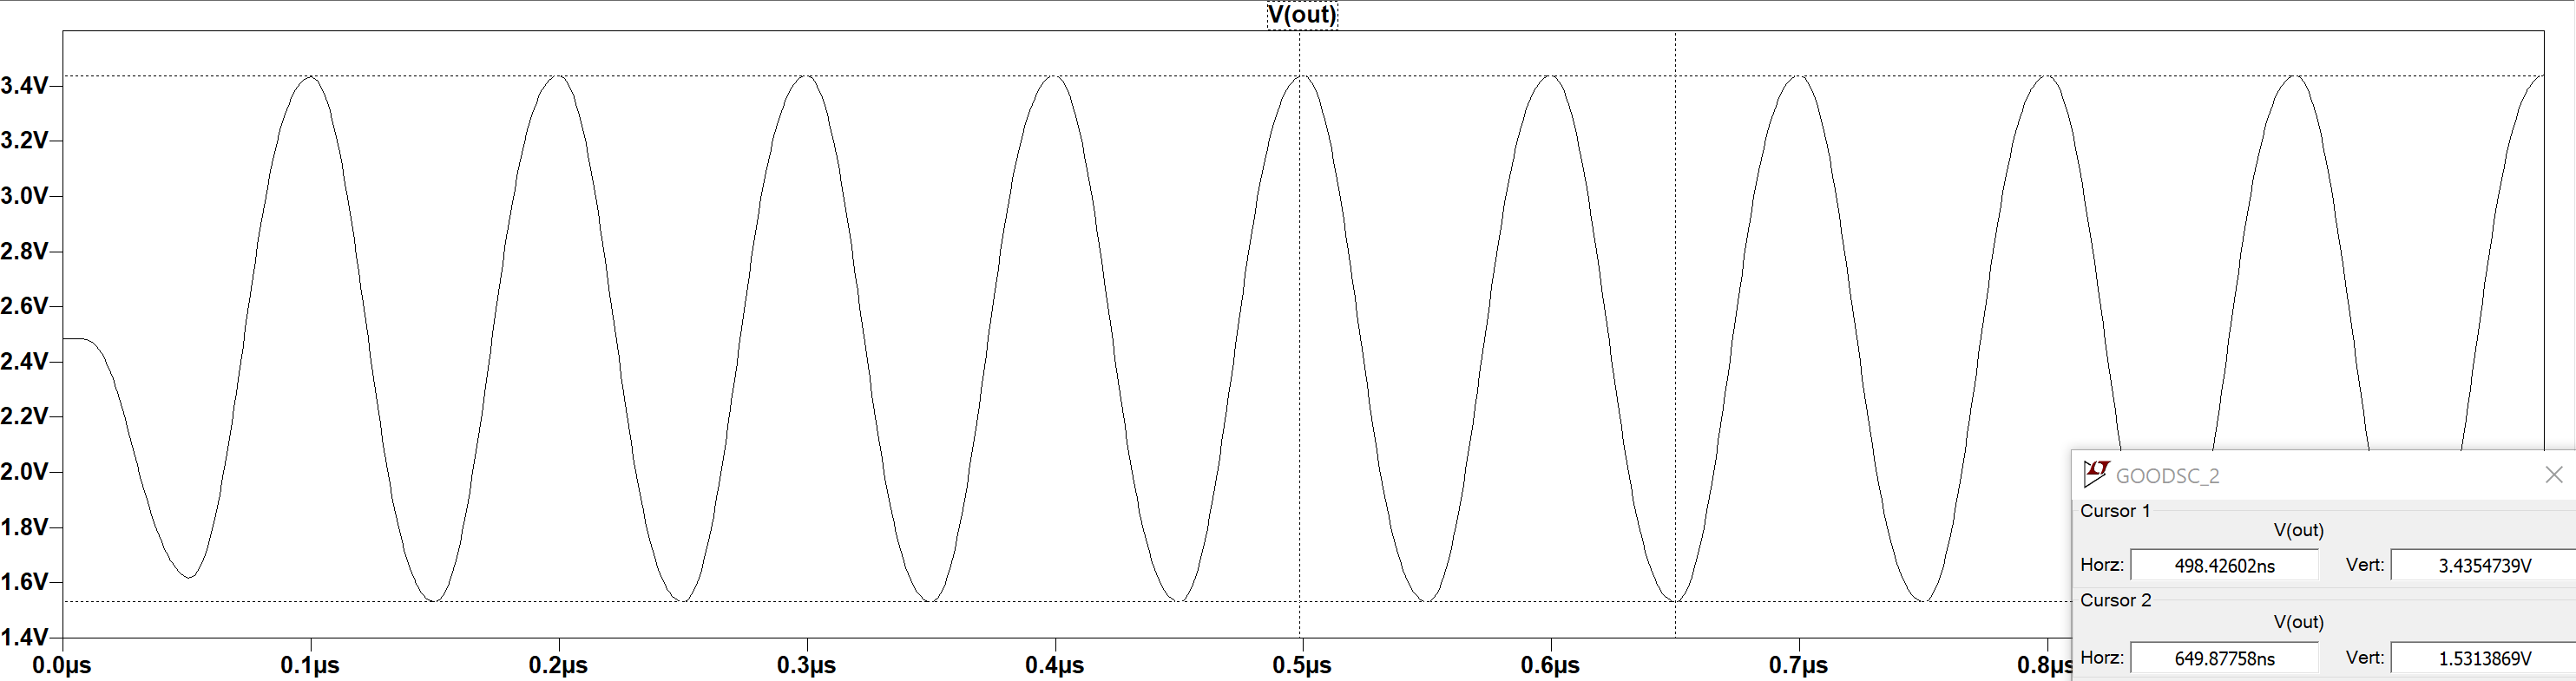
\includegraphics[width=16cm]{10M2.png}
\caption{Input to the ADC when apply a 10Mhz input with 7V amplitude.}
\end{figure}
From the figure above, the amplitude is still in control when a unproperly large signal is implemented.
\section{Circuits analysing and specification criteria}
\subsection{Input Protection}
\begin{figure}[H]
\centering
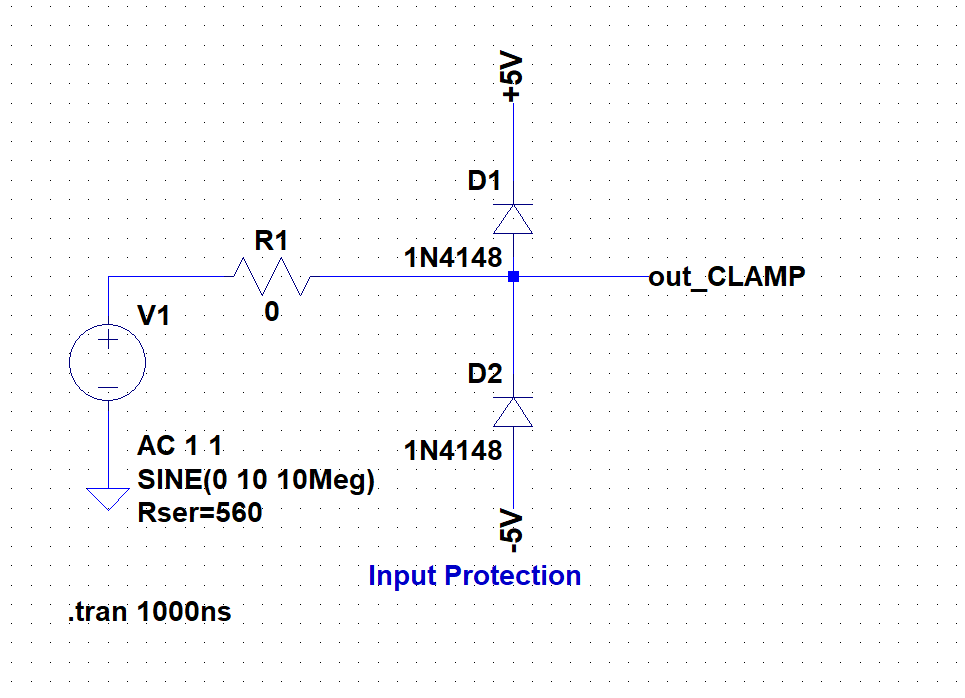
\includegraphics[width=10cm]{Protect.png}
\caption{Input protection circuit}
\end{figure}
~\\
To test the input amplitude protection, a $10V$ AC input is implemented. The output signal is shown as below. \textbf{The input signal is limited by two diode, and the maximum amplitudes are $\mathbf{5V+V_{on}}$ and $\mathbf{-5V-V_{on}}$, which from the plot is about $\mathbf{\pm 5.6V}$.}
\begin{figure}[H]
\centering
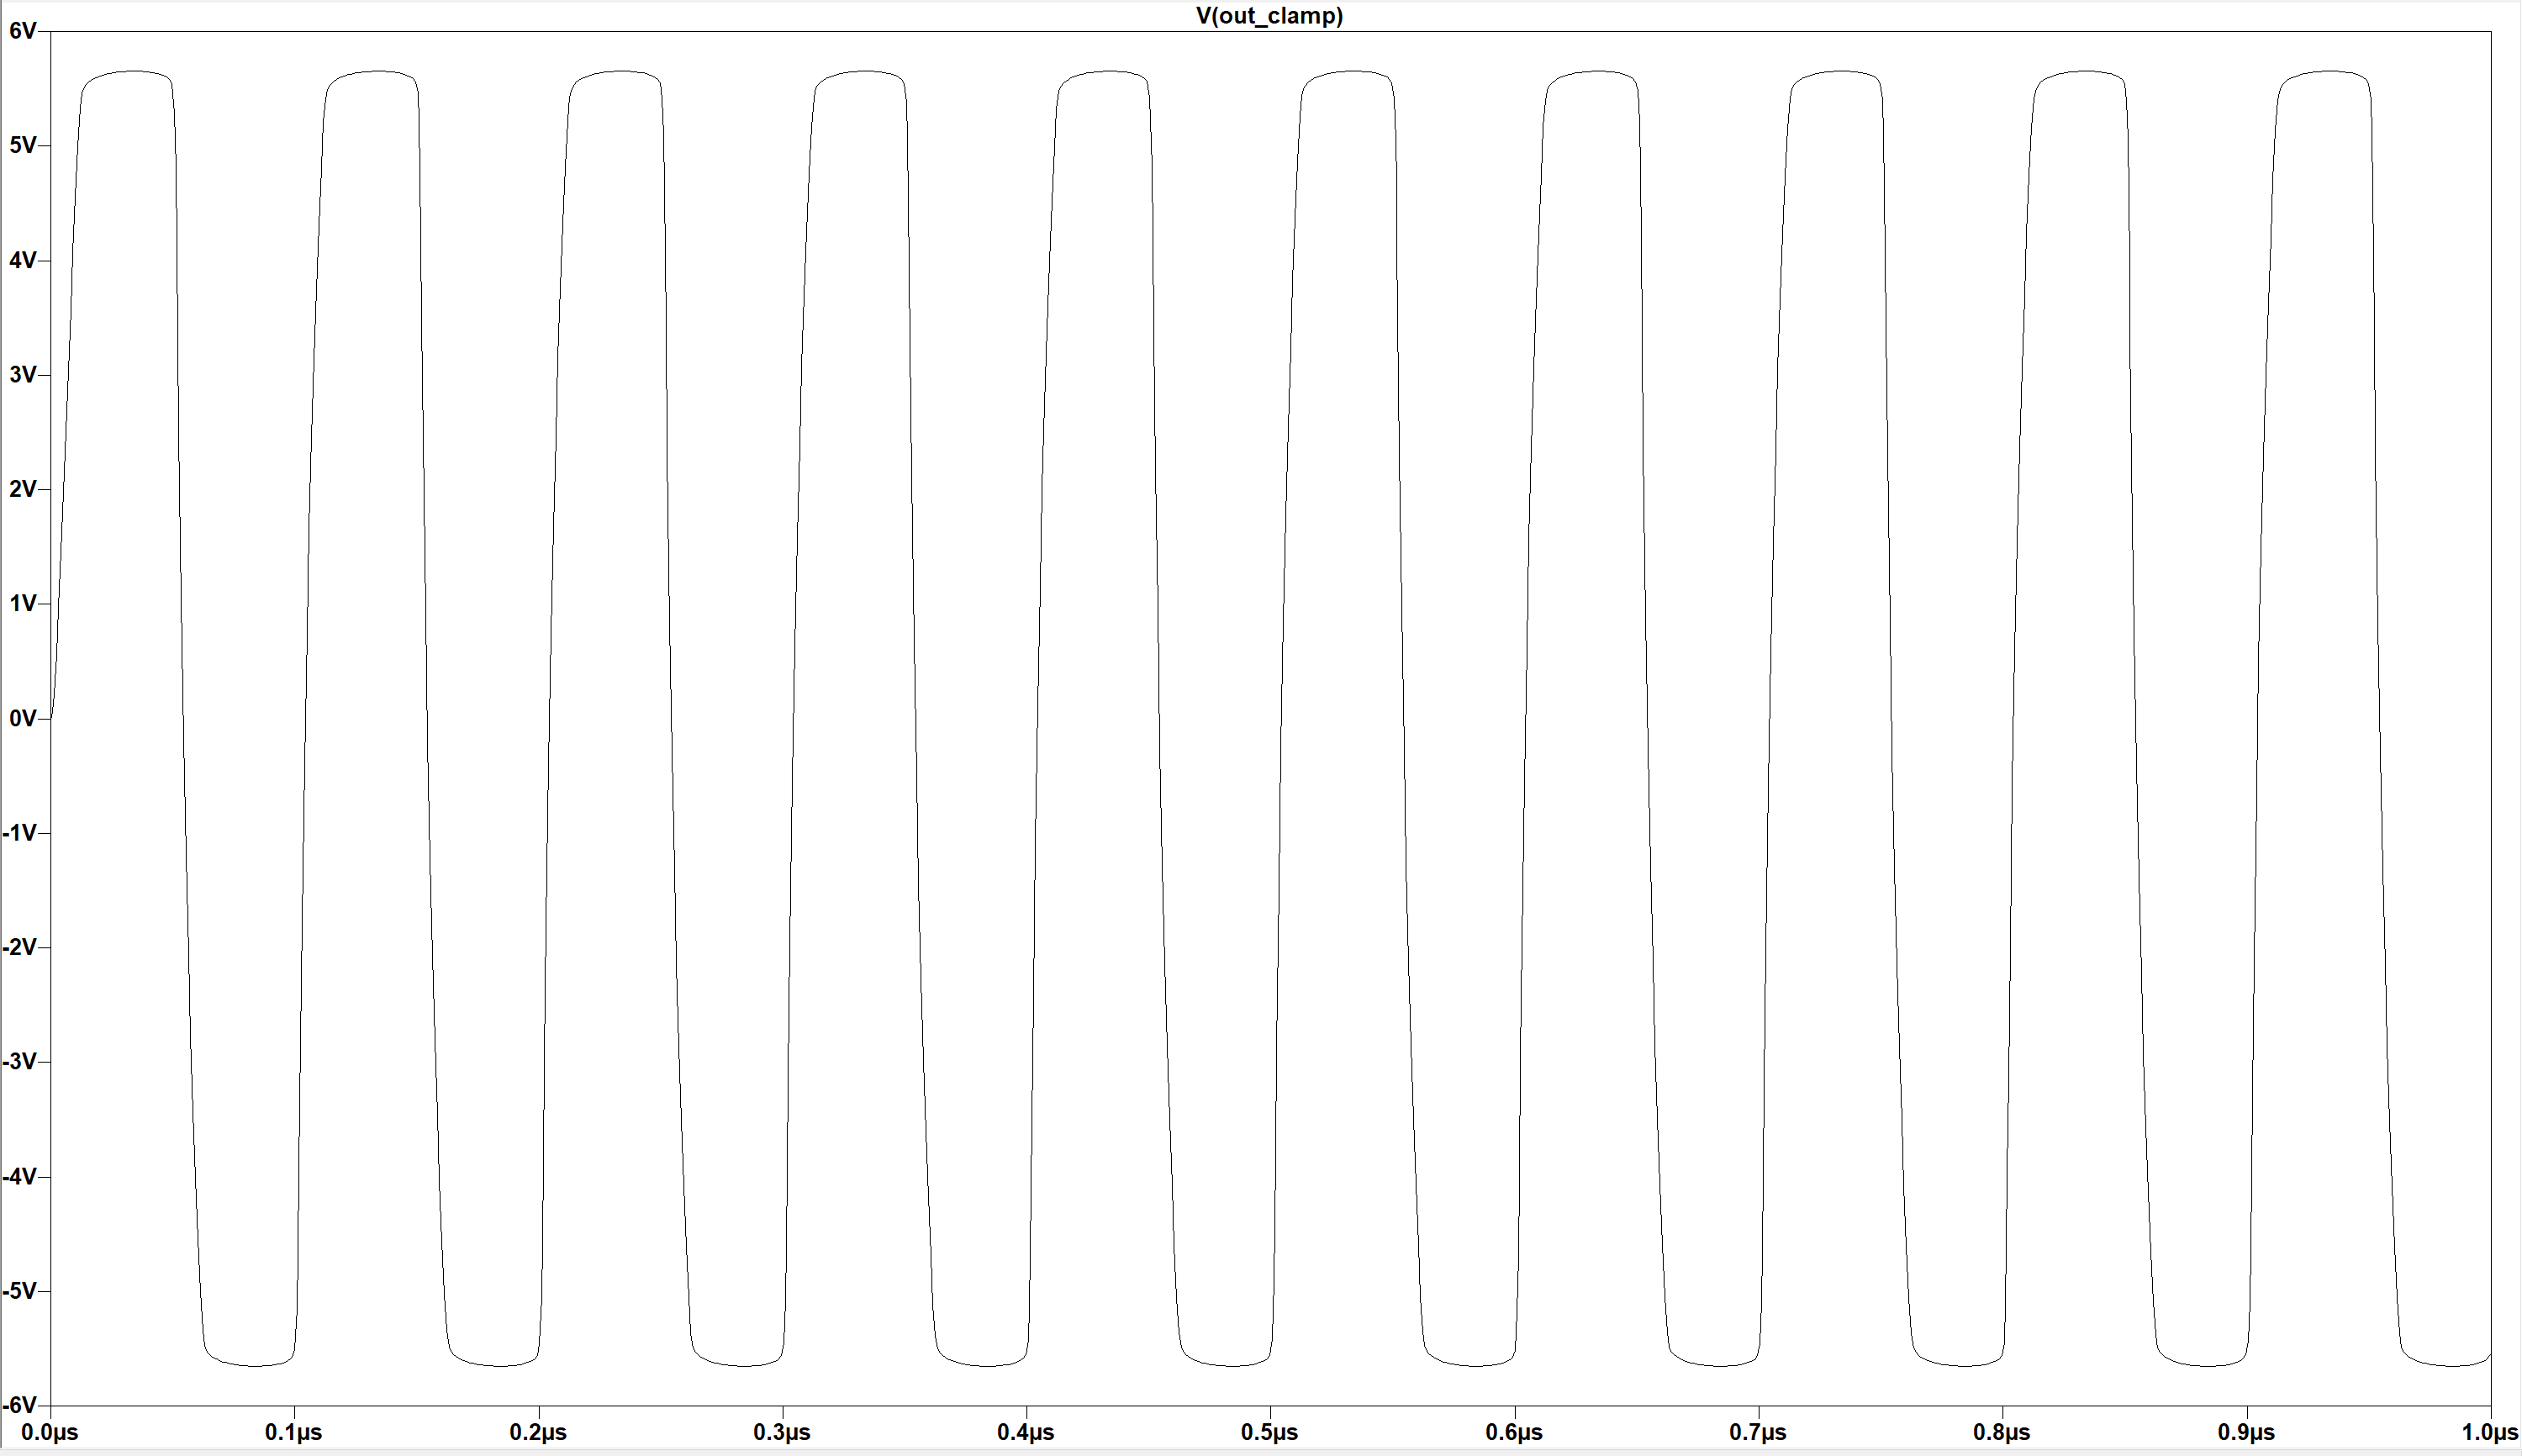
\includegraphics[width=10cm]{proout.png}
\caption{Output signal after the protection circuit}
\end{figure}
\subsection{Input impedance and buffer}
\begin{figure}[H]
\centering
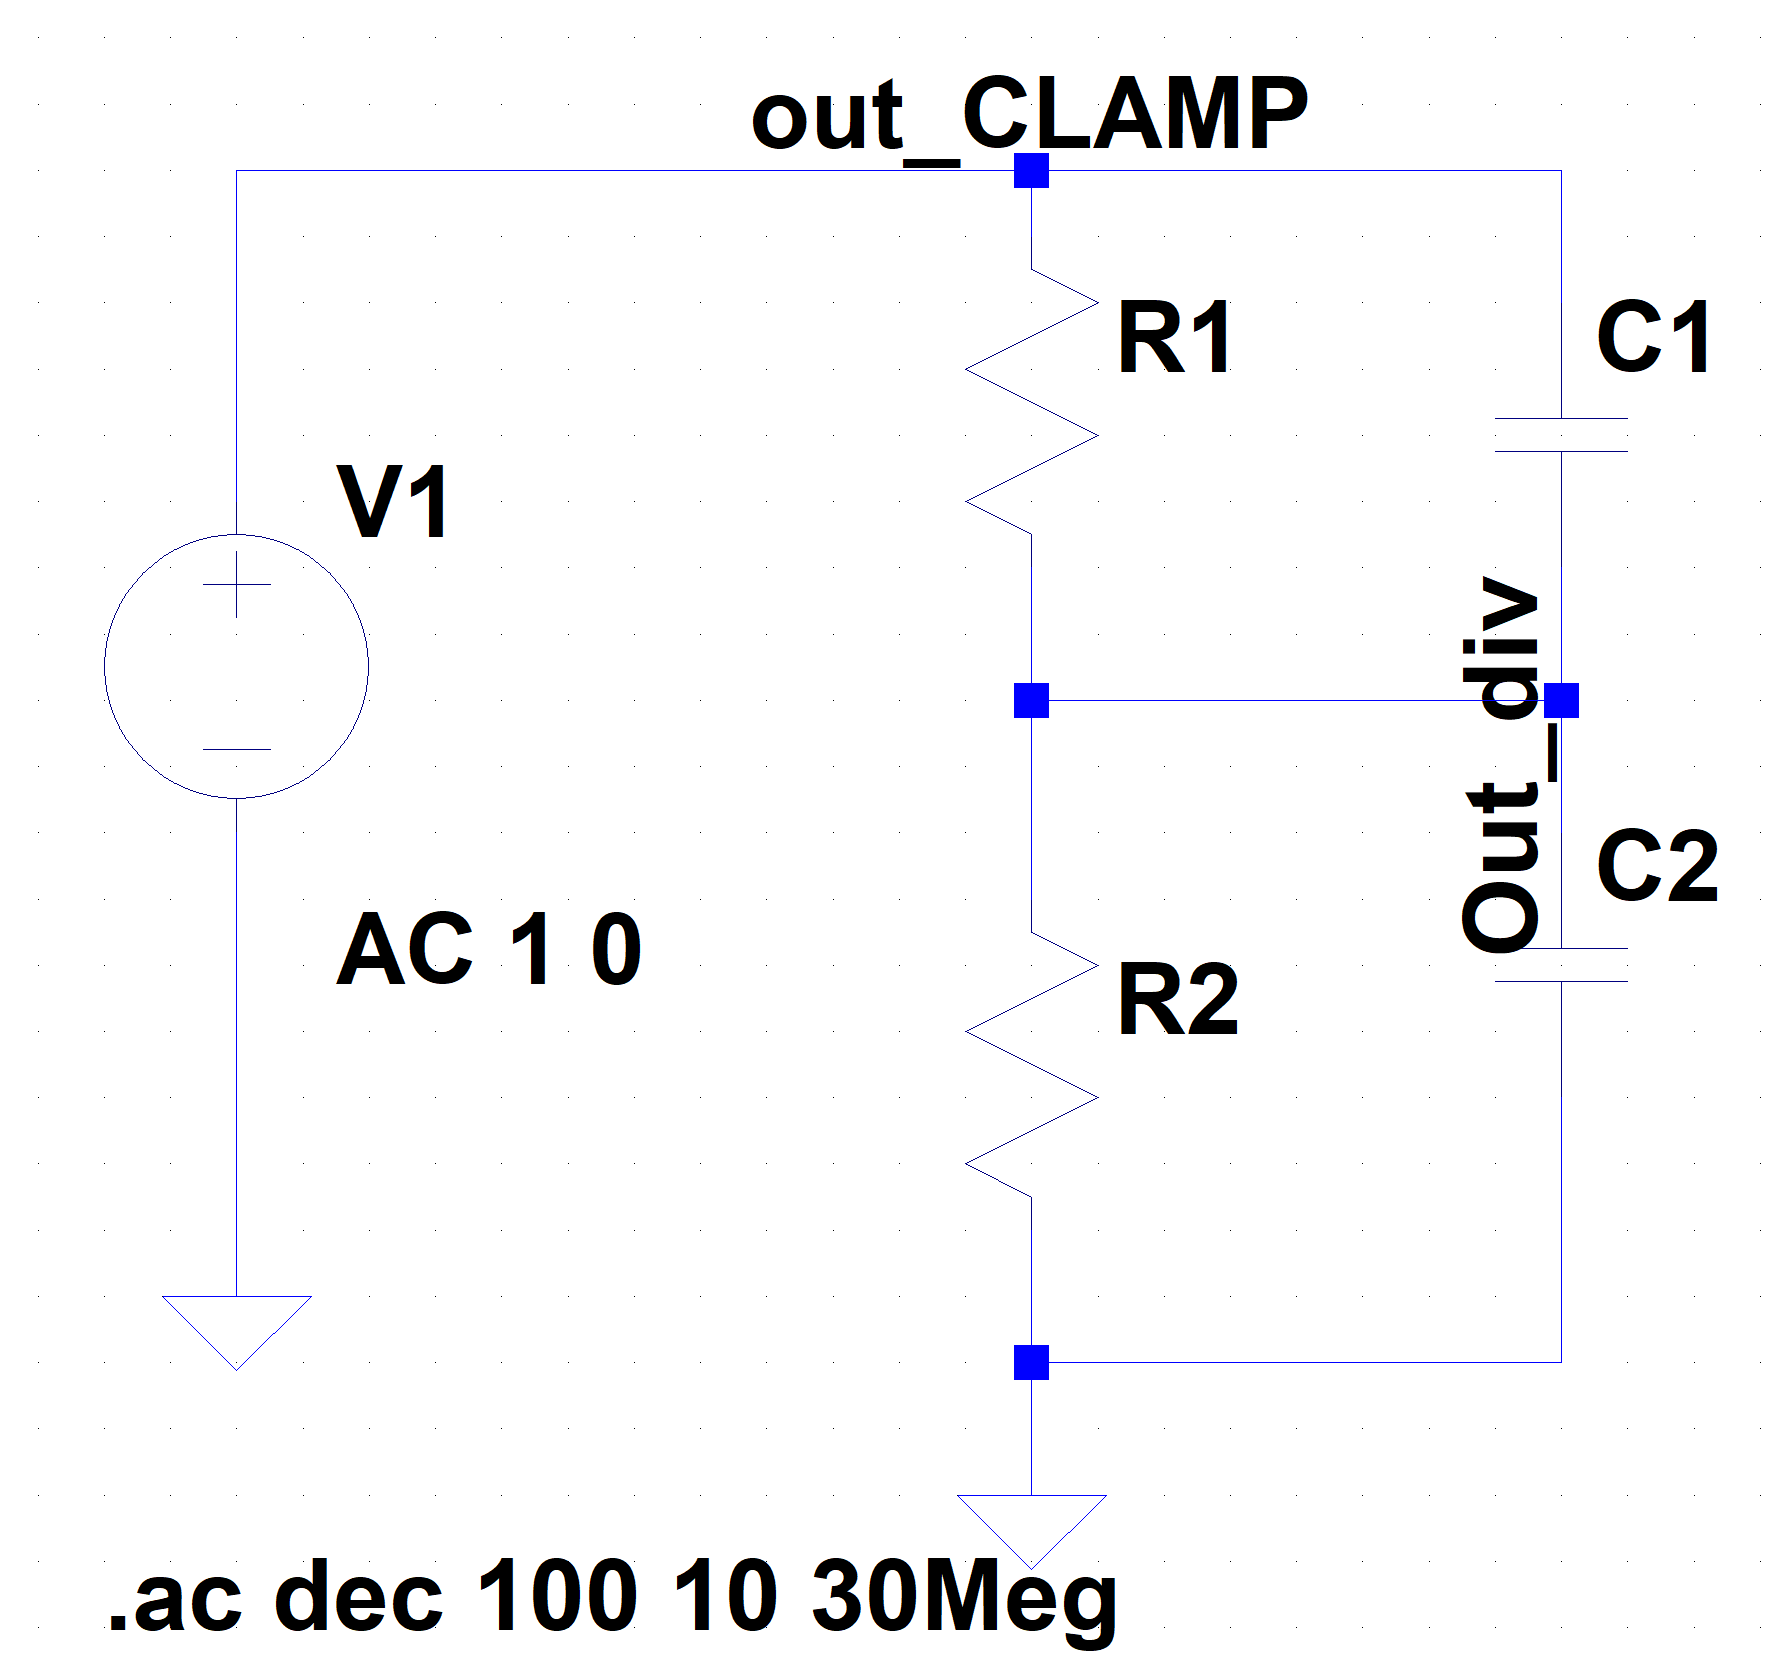
\includegraphics[width=6cm]{Input-imp.png}
\caption{Impedance components for the Front end circuit}
\end{figure}
~\\Since the construction above is between the protection circuit and the buffer, we can state this part is mainly used to provide a proper impedance for the circuit as the buffer isolate the impedance. Based on our functional specifications, \textbf{we need a $\mathbf{1M\Omega \pm 10\%}$ input impedance from DC to $\mathbf{10kHz}$, and greater than $\mathbf{100 ohms}$ between 10 kHz and 30 MHz. } Firstly, when a DC is implemented, C1 and C2 are open, hence we have $R1+R2=1M\Omega \pm 10\%$. Another factor we need to consider is the frequency response:
\begin{align}
\frac{V_{out-div}}{V_{out-CLAMP}}&=\frac{Z_2}{Z_1+Z_2}\\
&=\dfrac{R_2||\frac{1}{2\pi f C_2}}{R_1||\frac{1}{2\pi f C_1}+R_2||\frac{1}{2\pi f C_2}}\notag\\
&=\frac{R_1(1+sR_2C_2)}{R_1(1+SR_2C_2)+R_2(1+SR_1C_1)}\notag
\end{align} 
From the equation above, we have one zero and one poles. As zero brings 20dB increase per decade and poles brings 20dB decrease per decade, to get a flatter frequency response at all band, there are two possible ways. \textbf{One is that we need our pole and zero far bigger than $\mathbf{30Mhz}$}, which means $R_1C_1<<3\times 10^{-7}$. However, since the smallest capacitor we have is $1nf$ and the two impedance requirements make this method impossible. Another possible way is we put zero and poles locate at the same position. \textbf{Although this will still cause phase oscillation at some frequency, the overall frequency response is relevant stable} Hence:
\begin{align}
\frac{-1}{R_1C_1}&=-\frac{R_1+R_2}{R_1\cdot R_2(C_1+C_2)}\\
R_1\cdot C_1&=R_2\cdot C_2
\end{align}
To simplify the calculation. we assume $R_1=R_2$, so we can state $C_1=C_2$, the discussed part is a half divider. Hence $R_1=R_2\thickapprox 500K\Omega$. \textbf{The closet value available is $\mathbf{510k\Omega}$}. When the frequency affects the circuit, we have:
\begin{align}
Z_{in}&=2\times (R||\frac{1}{2\pi fC})\qquad R_1=R_2=R;\quad C_1=C_2=C\\
&=\frac{2R}{1+2\pi fCR}\notag
\end{align}
From the equation above, to achieve the functional specification, we need:
\begin{align}
\frac{2R}{1+2\pi fCR}&\geq 100\qquad R=510k\Omega\quad f=30\times 10^6\\
C& \leq 106pf
\end{align}
Another requirement here is \textbf{out input capacitance should be less than or equal to $\mathbf{60pF}$}. Under this condition, I put two ${5pf}$ small capacitors. Another reason is to guarantee the input impedance. Implement those parameter and plot the impedance as below:
\begin{figure}[H]
\centering
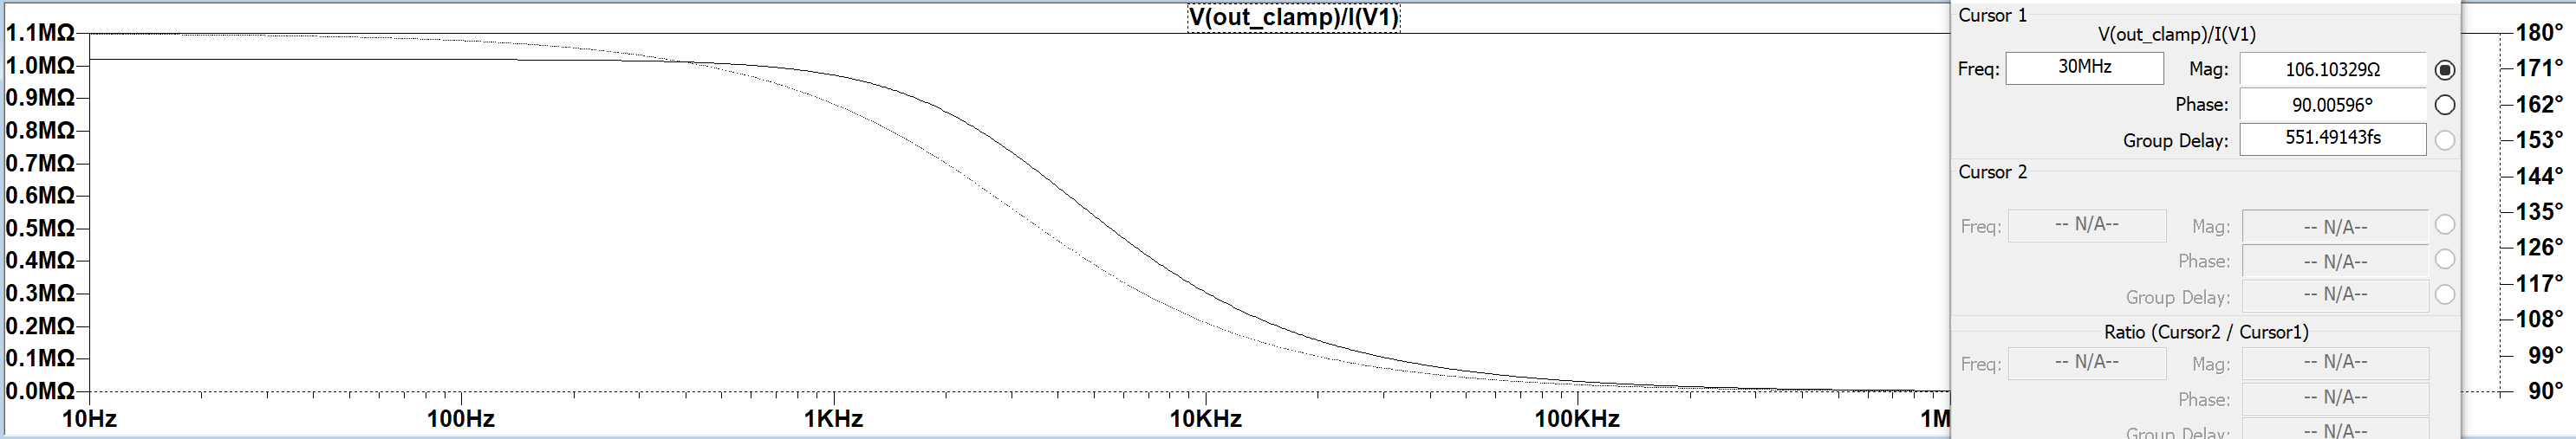
\includegraphics[width=17cm]{impedance.png}
\caption{Input impedance simulation}
\end{figure}
~\\From the figures above, \textbf{we can state our design satisfies the impedance requirements.}
Besides these, the slightly phase can be seen as below:
\begin{figure}[H]
\centering
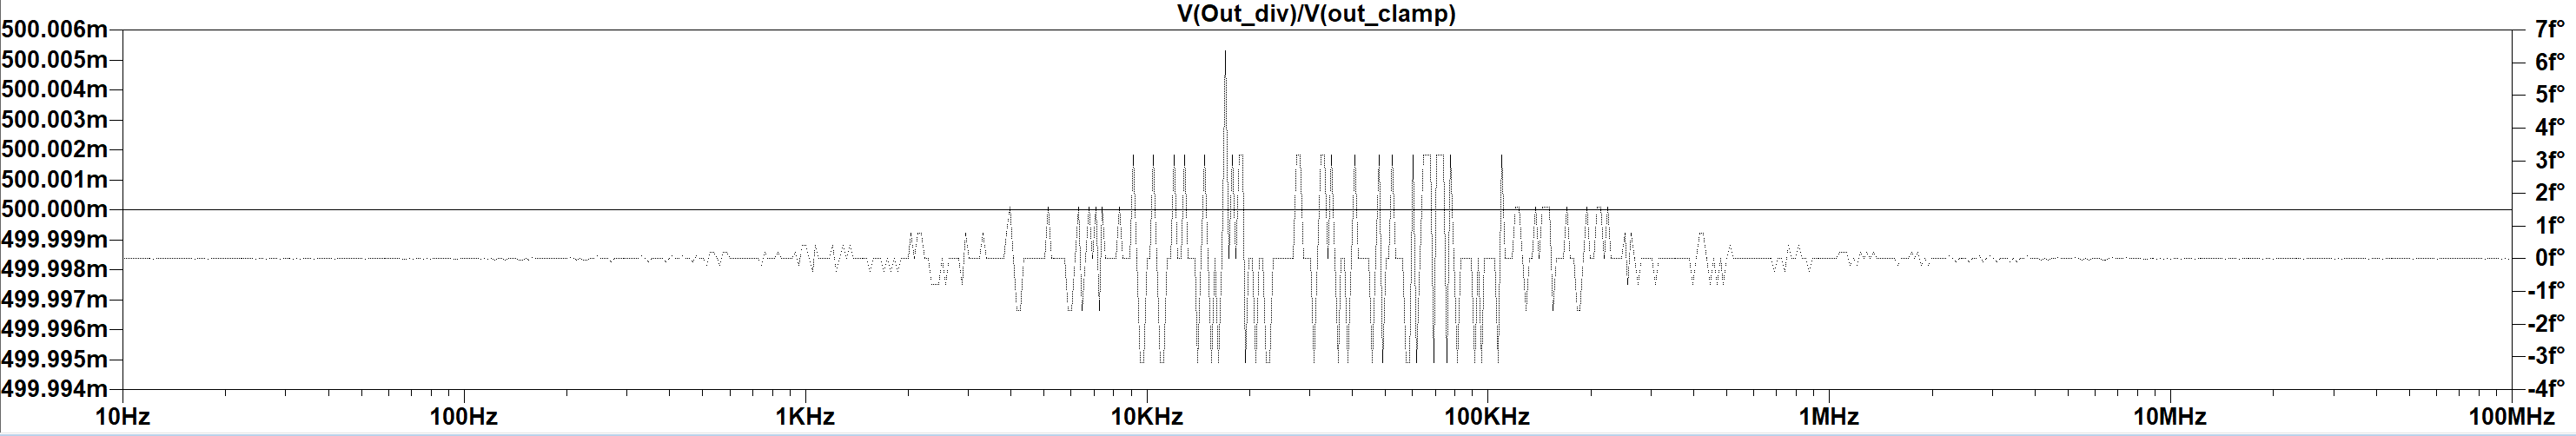
\includegraphics[width=17cm]{phase.png}
\caption{Constant gain and slightly oscillated phase}
\end{figure}
\subsection{Low pass filter}
The designed LPF is as below:
~\\Concretely, since the requirement 'An anti-aliasing filter appropriate to the $40MSPS$ maximum sample rate must be implemented with a minimum of a first-order $20dB$ per decade response and $\pm 2dB$ maximum ripple in the pass band' is expected to be meet. A second order Sallen Key Active Low Pass Filter then is used with reference circuit as figure 11. textbf{Since the gain is expected to be normal, the R4 is open.} Besides, based on sampling theorem, the cut-off frequency should be $20Mhz$, hence $f_0$ is set to $20Mhz$ to guarantee the bandwidth, and a is set to 1. 
\begin{figure}[H]
\centering
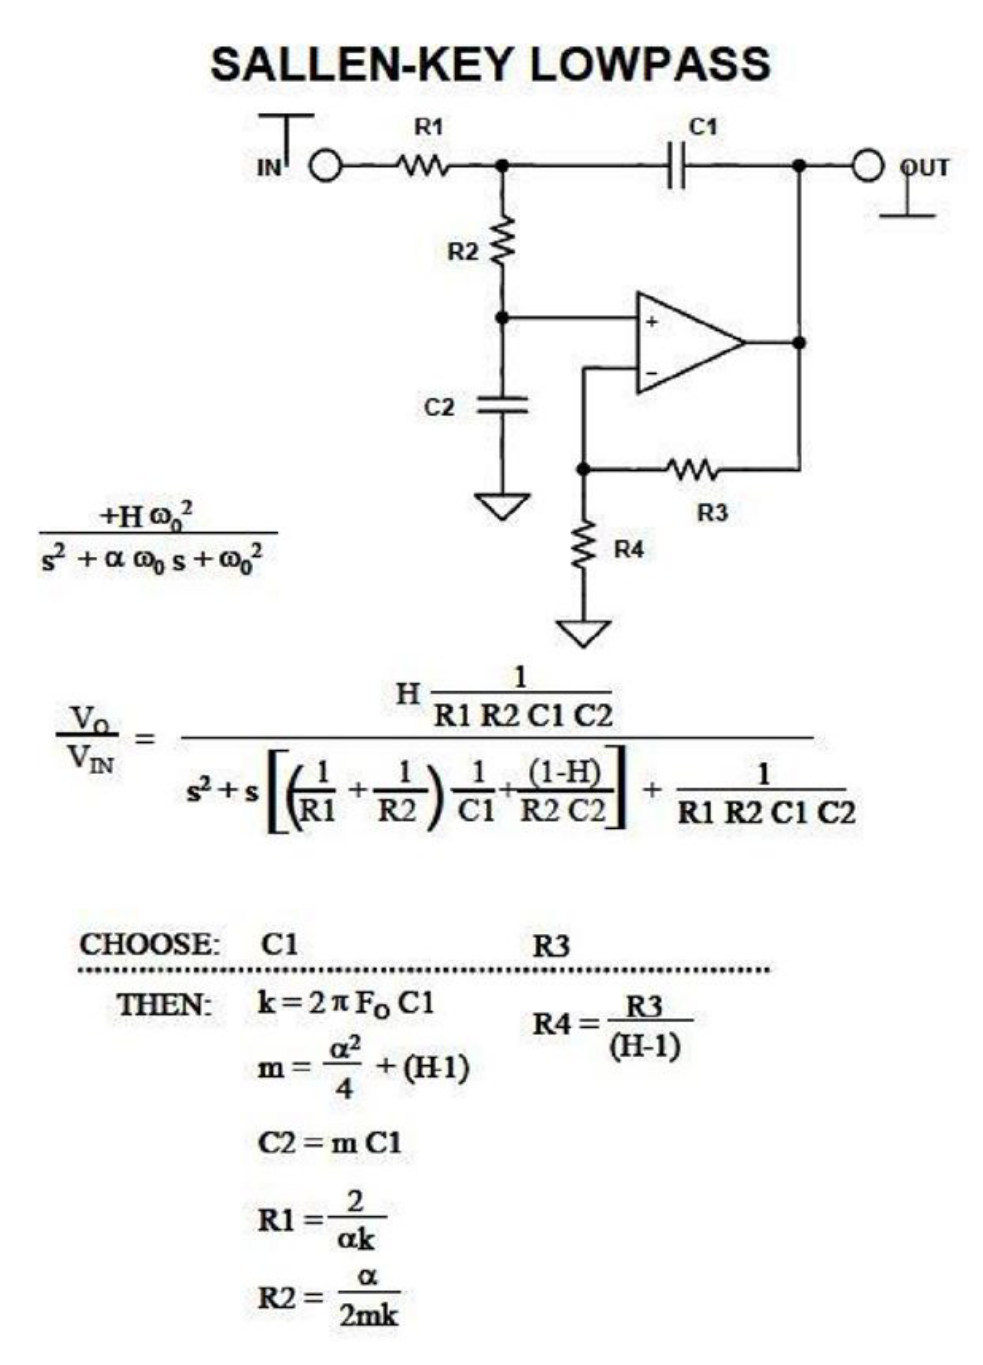
\includegraphics[width=12cm]{reff.png}
\caption{Given reference circuit and equation}
\end{figure}
~\\ After calculating based on the equations above, we built our LPF as below:
\begin{figure}[H]
\centering
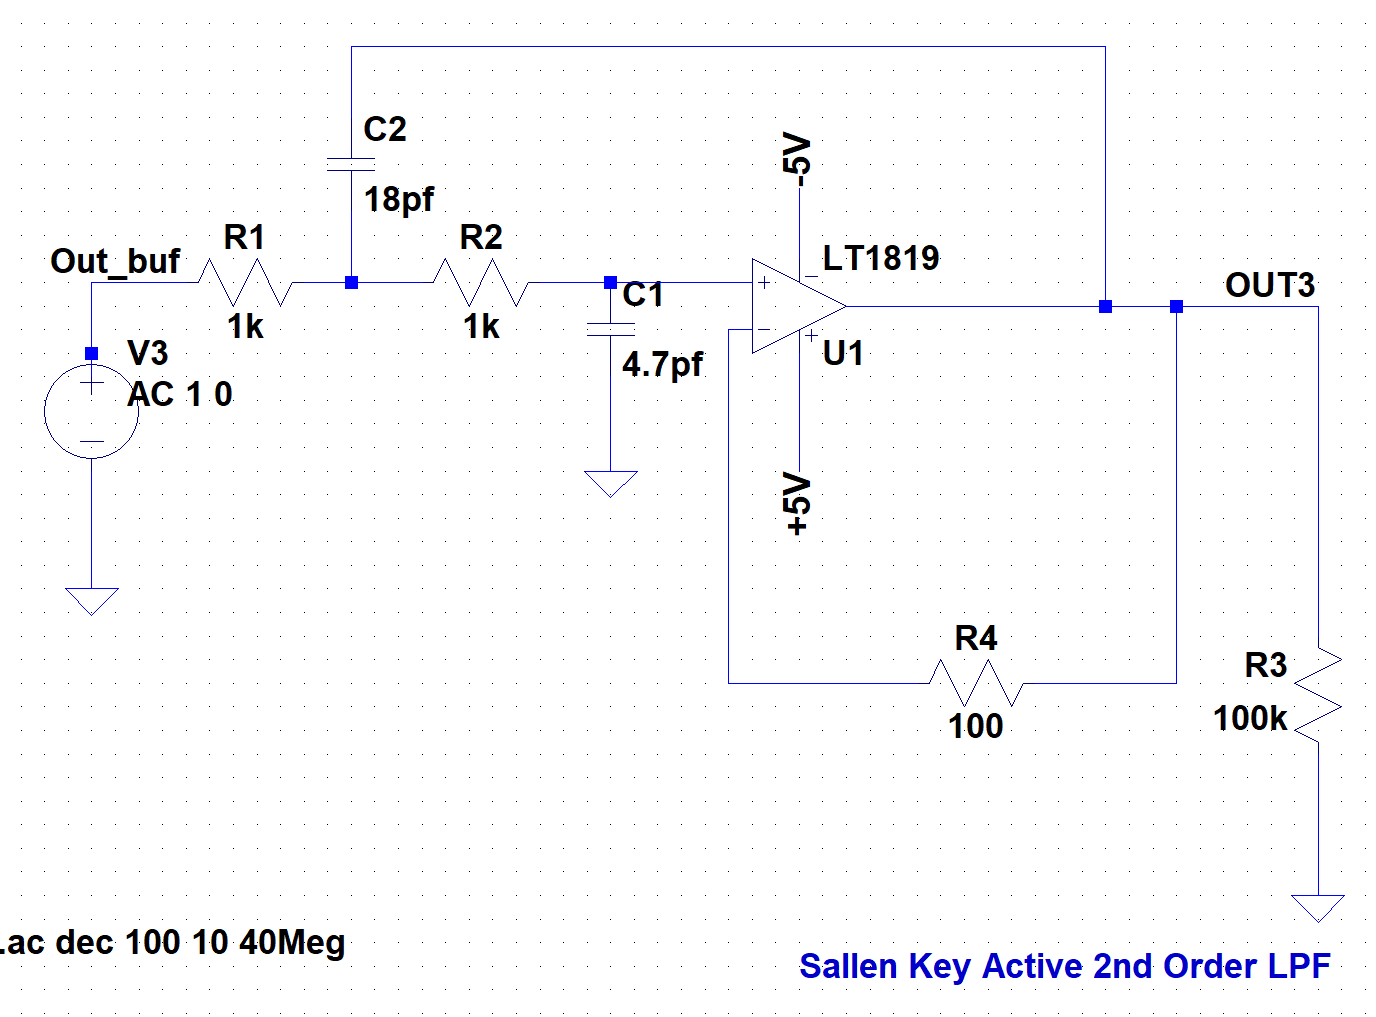
\includegraphics[width=12cm]{lpf.png}
\caption{Built low pass filter}
\end{figure}
~\\ To test the frequency response, a 1V AC input is plugged and the bode plot as below, although a much more larger bandwidth is generated, the final bandwidth is just a little bit more than we need as shown in figure 2:
\begin{figure}[H]
\centering
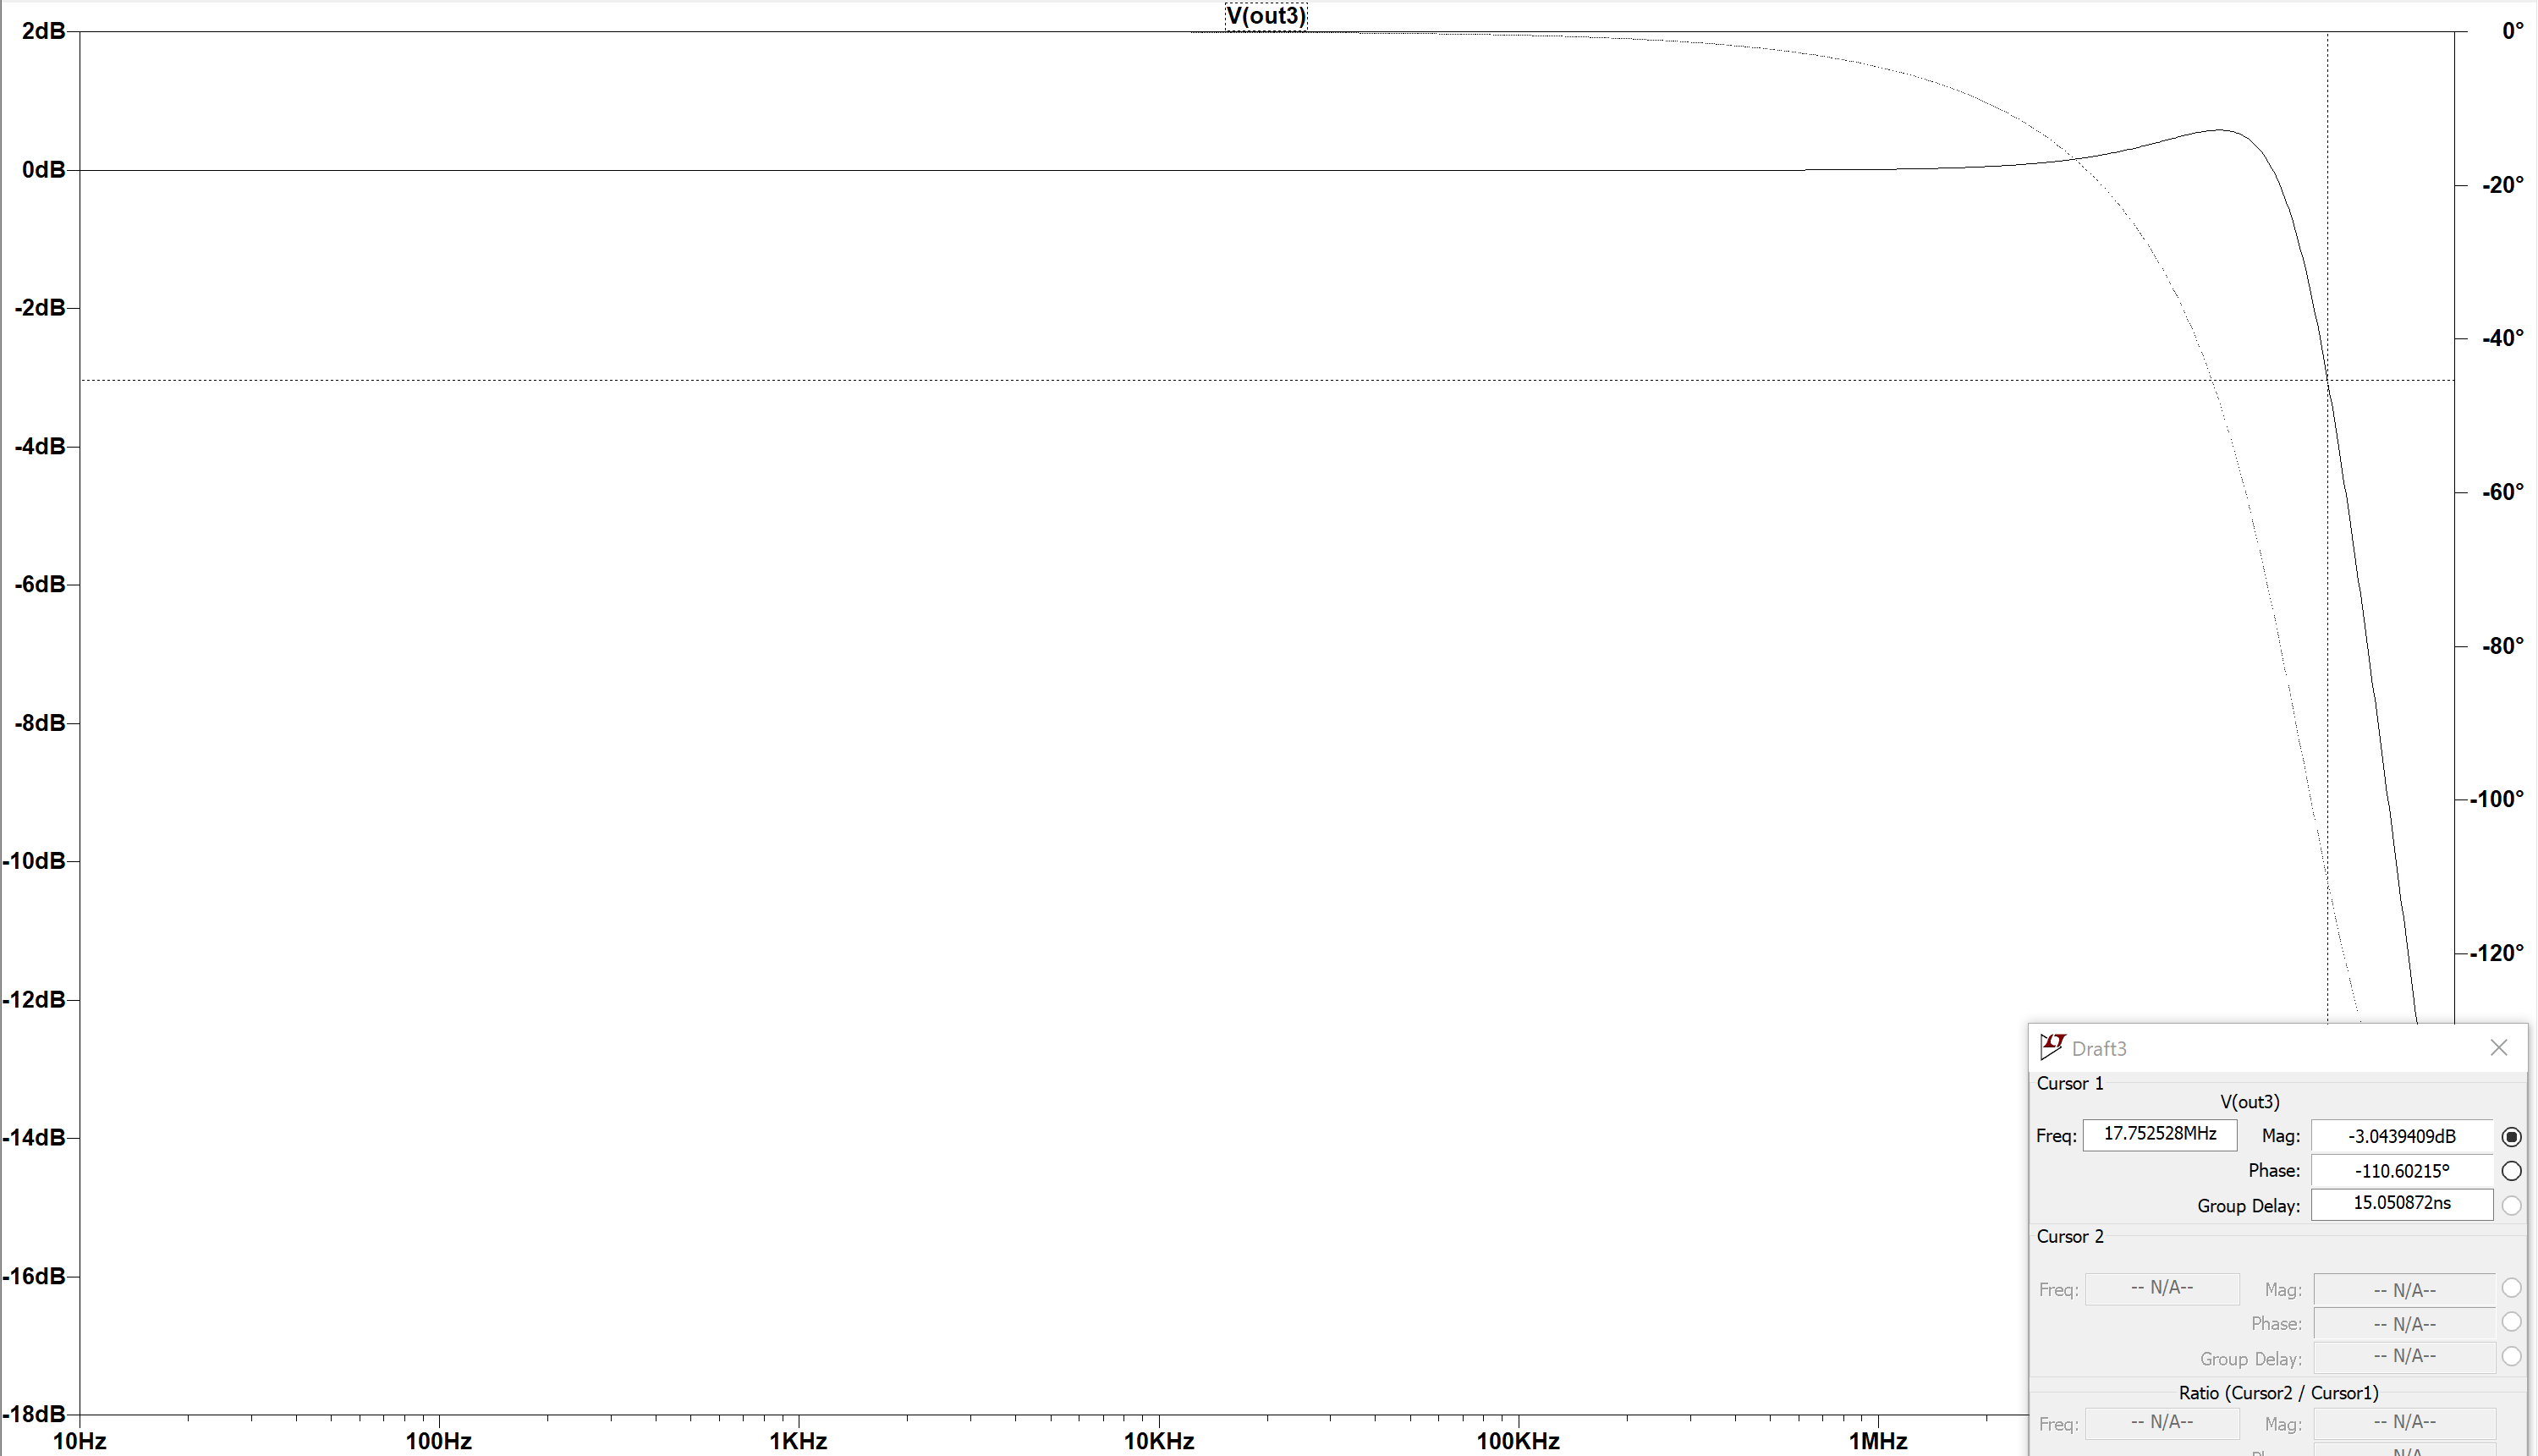
\includegraphics[width=12cm]{bode.png}
\caption{Bode plot of the low pass filter}
\end{figure}
\subsection{Gain stage and level shifting filter}
In this part, the circuit is divided to three part based on functions as comments illustrate below:
\begin{figure}[H]
\centering
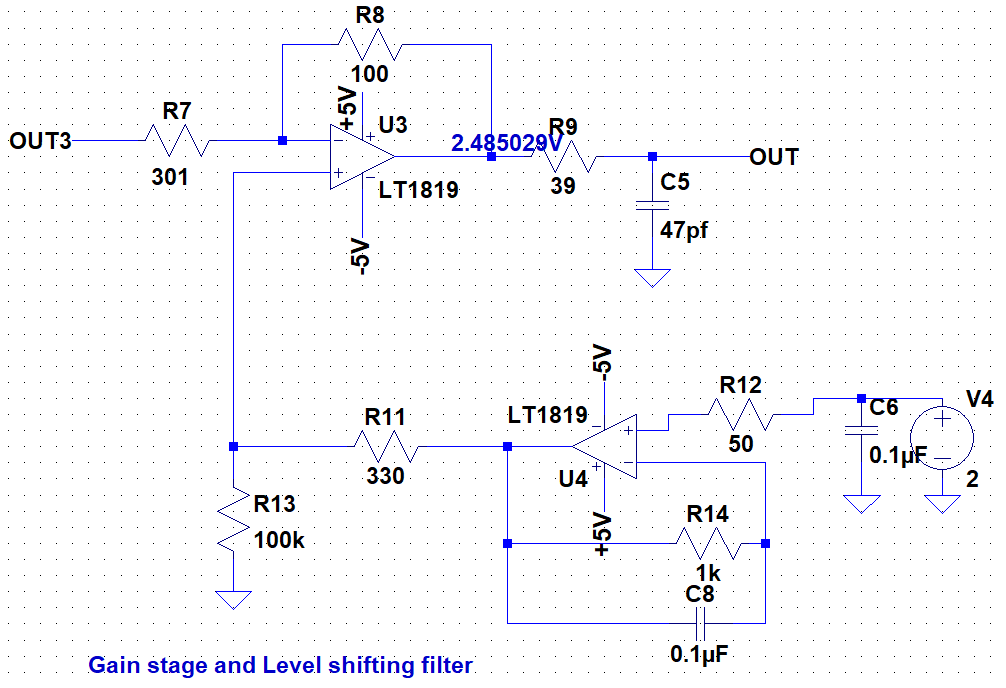
\includegraphics[width=12cm]{gainstage.png}
\caption{Gain stage and level shifting filter}
\end{figure}
~\\ From the bottom right to top left, a buffer is firstly used make sure our reference. Two resistors are used to bias our signals' center point to $5V$. However, this part is also affected by the gain stage, where we can scale the signal by changing resistor $R_1$ and $R_2$.\\
Yielding, the $R_2$ and $R_3$ is first calibrated to get a $\frac{2}{5.6}$ gain from outClamp to output3 in the figure 1 (The previous stages shrink the signal to a half as discussed above). Secondly, we change the level shifting to make central voltage at $2.5V$. As we have to select components form values supplied, the closet central point gotten is 2.48V. Then a $10Mhz$ test signal with 10V peak-to-peak is implemented to test the performance and the output is as figure 5.    
\section{Specifications Summary}
In conclusion, as discussed, we have meet the requirements below:
\begin{itemize}
\item \bf{The input impedance is above $\mathbf{9M\Omega}$ from 0 to 10hHz and above $\mathbf{100}$ between 10 kHz and 30 MHz.}
\item \bf{The input capacitance is less than 60pF}
\item \bf{The input signal can be champed to $\mathbf{\pm 5.6V}$ }
\item \bf{The signal path from the BNC input to the ADC shall be DC coupled.}
\item \bf{The lpf is anti-aliasing which support maximum 35MSPS sample rate, with a minimum of a first-order 20dB per decade response and $\mathbf{\pm 2dB}$ maximum ripple in the pass band}
\item \bf{All passive components are selected based on values supplied.}
\end{itemize}
\end{document}